\documentclass[noposter]{polytech/polytech}

\newcolumntype{L}[1]{>{\raggedright\arraybackslash}p{#1}}

\typereport{prddi5}

\reportyear{2018-2019}
\title{Outil de gestion de parcours patient dans un hôpital de jour}
\student[di5]{Romain}{ROUSSEAU}{romain.rousseau@etu.univ-tours.fr}
\academicsupervisor{Yannick}{KERGOSIEN}{yannick.kergosien@univ-tours.fr}

\resume{Les hôpitaux sont l'objet de nombreux débats dans l'actualité, et l'un des points de discussion principal est la gestion des patients au sein des établissements. Un projet de développement d'une plateforme permettant de planifier les rendez-vous des patients au sein d'un hôpital de jour a été réalisé lors des années précédentes par des étudiants de l'école. La plateforme permet de gérer les patients, de leur assigner ce qu'on appelle un parcours patient, et d'agencer leur planning selon les ressources disponibles. Je vais reprendre ce projet pour corriger les divers problèmes présents et pour implémenter la planification automatique des activités des patients. Ajouter une planification automatique implique de nombreuses questions qui seront évoquées dans ce rapport.}

\motcle{plateforme, web, gestion, patients, planification automatique}

\abstract{Hospitals are subject to numerous talks in the news, and one of the main point is about the scheduling of patients. The creation of a platform allowing users to schedule patients activities in the hospital was made by student of the school in the years before. The application allows to add patients and resources, to assign them a course to follow, and to schedule with the resources available. I will continue this project by first, correct some bugs in the platform and to add automatic scheduling. The automatic scheduling implies lots of questions which will be answered in this report.}

\keyword{platform, web, management, patients, automatic scheduling}

\posterblock{Contexte}{Les hôpitaux cherchent de nouvelles solutions pour aider la gestion des patients. Une plateforme a déjà été réalisée par les élèves de l'école lors des années précédentes et permet d'attribuer des parcours aux patients afin d'agencer leur rendez-vous sur un calendrier de façon manuel.}{images/LOGO_APHP}{Logo de l'Assistance Publique Hôpitaux de Paris}

\posterblock{Objectifs}{Mes objectifs seront de corriger les erreurs présentes sur la plateforme, notamment des erreurs d'affichage, des fautes d'orthographe, des problèmes de modélisation. Une fois corrigé, l'objectif sera d'implémenter une planification automatique des patients permettant, en un clic, d'avoir les rendez-vous programmés pour le jour donné.}{images/planningPatient}{Affichage d'un planning patient vide}

\posterblock{Fonctionnalités}{
	\begin{itemize}
		\item Amélioration générale apportée à la plateforme
		\item Implémentation de la planification automatique
	\end{itemize}
}{images/bouton_plan_auto}{Aperçu de la page de planification}


\addbibresource{PRD2.bib}

%%%%%%%%%%%%%%%%%%%%%%%%%%%%%%%%%%%%%%%%%%%%%%%%%%%%%%%%%%%%%%%%%%%%%%%%%%%%%%%%%%%%%%%%%%%%%%%%%%%
%%%%%%%%%%%%%%%%%%%%%%%%%%%%%%%%%%%%%%%%%%%%%%%%%%%%%%%%%%%%%%%%%%%%%%%%%%%%%%%%%%%%%%%%%%%%%%%%%%%

\begin{document}

\chapter*{Introduction}

Ce rapport traite du projet Recherche et Développement réalisé au sein de l'école Polytech. Il se déroule lors la cinquième année d'étude et représente une forme de synthèse des connaissances acquises lors des années d’études précédentes. Il permet de développer et d'approfondir son savoir sur un ou plusieurs champs de compétences spécifiques, afin de devenir un spécialiste du domaine choisi dans le cadre du projet. Ce travail est mené seul, sous la supervision d'un tuteur académique et, pour certains projets, avec l'aide d'un intervenant extérieur qui fait partie des initiateurs du sujet. Il permet ainsi de développer son autonomie en menant à bien un travail des prémices jusque, dans le meilleur des cas, à la production.

J'ai décidé de me consacrer à un projet lié à un enjeu important de notre société: la gestion des patients dans un hôpital. Aujourd'hui, les hôpitaux sont l'objet de nombreux débats dans l'actualité, et l'un des points de discussion majeurs concerne la gestion des patients au sein des hôpitaux. Plusieurs problèmes peuvent être cités: un temps d'attente bien trop long pour les patients (que ce soit une fois à l'hôpital ou pour avoir un rendez-vous avec un spécialiste), des problèmes de ressource (concernant le personnel ou bien les salles à disposition) ou encore des problèmes d'ordre financier en général. Certaines de ses problématiques peuvent être étudiées selon le point de vue de l'optimisation, et la recherche opérationnelle peut permettre d'améliorer certains aspects de la gestion actuelle. Pour ma part, me pencher sur les problèmes de recherche opérationnelle en général m'intéressait, et avoir l'opportunité de réaliser un projet dans ce domaine, d'autant plus dans un secteur qui en a besoin, était une bonne occasion pour améliorer mes compétences.

Le sujet de ce travail rentre dans le cadre d'un projet visant à développer un outil de gestion temps réel de parcours de patients pour l’AP-HP (Assistance publique - Hôpitaux de Paris). L'objectif de cet outil est de gérer un ensemble de patients nécessitant plusieurs activités de soins planifiées sur une journée dans un hôpital de jour. Chaque patient doit suivre un « parcours de soins » défini par un ensemble d'activités de soins. Certaines doivent être réalisées avant d'autres (contraintes de précédences) alors que pour d'autres, l'ordre n'a pas d'importance. Il peut exister des délais d'attente à respecter entre les activités. Chaque activité de soin est caractérisée par une durée et un ensemble de ressources nécessaires pour la réaliser. Ces ressources peuvent représenter le personnel, la salle où s'effectue l'activité ou encore le matériel utilisé. Elles sont caractérisées par une quantité et un horaire où elles sont disponibles. L'idée de l'outil est de pouvoir proposer un calendrier adaptatif dans lequel les horaires des activités de soins des patients peuvent être ajustés en fonction des aléas potentiels (retard, patient absent, etc.) afin de diminuer au mieux possible le temps d'attente des patients.

Ce projet est la suite de plusieurs travaux effectués à l'école Polytech ces dernières années et qui ont abouti à une première version simple d'un outil sous forme de plateforme web. L'objectif est d'améliorer l'outil actuel en corrigeant certains problèmes et en ajoutant des fonctionnalités afin de se rapprocher d'une version finale exploitable à l'avenir. Parmi les fonctionnalités qui devront être ajoutées, on peut notamment penser à la planification automatique des activités de soin sur le calendrier ou encore l'ajout de notions de temps réel sur les éléments du calendrier.

La première partie de ce rapport sera consacrée à l'analyse préliminaire de la plateforme et à la détermination des tâches à réaliser. Elle comprend des éléments sur le contexte de la réalisation, la description de la plateforme telle qu'elle se trouvait au début du projet, un état de l'art sur les modélisation de la planification automatique des activités, et la présentation des tâches qui seront effectuées durant les semaines de projet. La seconde partie sera dédiée aux détails des développements de la plateforme. Des documents complémentaires sont disponibles en annexe de ce rapport comme les diagrammes de Gantt, les diagrammes UML, des éléments de gestion de projet, etc. 

%TODO PARTIE 2
%Un guide développeur destiné aux personnes qui désireront reprendre le projet à l'avenir est également présent en complément.


\part{Analyse préliminaire et détermination des objectifs}


Cette partie correspond à la première phase du Projet Recherche et Développement, la partie Recherche. Dans le cadre de ce projet, cette partie sera une analyse générale de la plateforme existante afin de déterminer quels objectifs nous devrons atteindre à l'issue de ce projet. Le premier chapitre sera consacré au contexte de la réalisation, la raison de l'initiation du projet ainsi que les acteurs concernés. Le chapitre suivant décrira la plateforme telle qu'elle se trouvait à la reprise du sujet, en détaillant la structure et les fonctionnalités qui existent. Enfin le dernier chapitre évoquera des éléments de recherche opérationnelle dans le domaine de la gestion des patients dans un hôpital. 


\chapter{Contexte de la réalisation et objectifs}
\label{chap:contexte}

Ce chapitre présente le contexte du sujet et les objectifs à atteindre à l'issue du projet.

\section{Contexte, enjeux et acteurs}

La santé dans notre société est un sujet prédominant dans l'actualité. De nombreux débats existent concernant la modernisation des structures hospitalières et surtout, la réduction des dépenses dans le secteur. Cependant, ces problématiques sont très complexes à gérer car il est important de maintenir une certaine qualité d'accueil nécessaire au bon traitement des patients, néanmoins une baisse des dépenses pourrait se répercuter dans la qualité des prestations. L'un des aspects sur lesquels ce projet sera consacré est la gestion de prise de rendez-vous médicale. Les consultations sont soumises à de nombreux aléas, que ce soit côté patient comme côté médecin. Il n'est pas rare pour un patient de devoir attendre plusieurs mois avant d'avoir un rendez-vous chez un spécialiste, tout comme il est fréquent pour un médecin de se retrouver avec un patient absent lors d'un rendez-vous. Ceci entraîne de la frustration et du gaspillage de ressources en général. Des solutions dans le domaine de la recherche opérationnelle peuvent être mises en place, afin d'améliorer la gestion des ressources médicales et de réduire les temps d'attente pour les patients, que ce soit avant ou pendant la prise en charge. 

Les services hospitaliers sont souvent surchargés par le nombre de patients dans l'établissement. Il est de plus en plus fréquent de voir les hôpitaux proposer des services en ambulatoire, c'est-à-dire prendre en charge un patient sur une seule journée, évitant ainsi les frais pouvant s'appliquer lorsqu'un patient dort sur place. Les dépenses liées aux hospitalisations sont parmi les plus importantes dans un établissement et de nos jours, les hôpitaux proposent même des alternatives pour que les patients ne restent pas sur place la nuit, comme par exemple des chambres d'hôtel afin de ne pas occuper une chambre pendant l'hospitalisation \cite{noauthor_chu_nodate}. Un établissement, ou une partie d'établissement, proposant ce type de service est appelé "hôpital de jour".

L'idée d'implémentation d'un outil numérique dans une structure implique une réflexion sur les concepts liés l'hospitalisation d'un patient. Il est possible de définir, selon les pathologies à traiter, un parcours-patient à suivre. Un parcours-patient (ou parcours-clinique) est un plan de soins pluridisciplinaires exposant les étapes que doivent un patient pour un problème spécifique. On peut les décomposer en plusieurs activités prédéfinies, certaines devant être réalisées avant d'autres (ce qu'on appelle une contrainte de précédence), nécessitant des ressources physiques ou matérielles (contrainte de ressources) et devant être effectuées dans un délai ou un créneau horaire précis (contrainte temporelles). La mise en place d'un système de centralisation des parcours-patient reste difficile, notamment car elle repose en priorité sur une bonne communication entre les services d'un établissement. Néanmoins, cela permettrait d'avoir potentiellement une meilleure utilisation des ressources de l'hôpital et par conséquent, un effet favorable sur les durées d'hospitalisation et les dépenses hospitalières entre autres.

L'Assistance Publique - Hôpitaux de Paris (AP-HP), dans son plan stratégique 2015 - 2019, a lancé une réflexion sur la mise en place d'une clinique ambulatoire. Avec la mutualisation de certains services au sein de différents hôpitaux de la région, le site de l'hôpital \textit{Béclère}, situé dans la ville de Clamart dans le département des Hauts-de-Seine, obtiendra un gain de place suffisant pour proposer une telle solution. Il regroupera tous les hôpitaux de jour existants du site, avec un management centralisé et transversal à l'aide de parcours-patients. Les équipes médicales et administratives ont pris le soin de définir d'ors et déjà une vingtaine de parcours patients en adéquation avec les ressources déjà en place, et présenté une répartition type des prises en charge hebdomadaire. Celle-ci devrait en théorie permettre d'accueillir 179 patients chaque semaine, et à terme environ 1000 par mois. Ainsi, la conception d'un système d'aide à la décision pour la prise de rendez-vous serait utile pour une nouvelle structure comme celle-ci.

Le sujet a été proposé en 2015 par Lucie ROUSSEL, ingénieur en ordonnancement à l'AP-HP et a été suivi lors de plusieurs projets à Polytech: tout d'abord, lors d'un projet collectif (réalisé par les étudiants Benjamin COLMART, Jean COQUELET, Anaëlle HAMON, Jiang MING, Yan LI et Minghui ZHANG) qui a posé les bases de la modélisation et des premières fonctionnalités, un projet R\&D effectué par Jean COQUELET en 2016 également basé davantage sur l'aspect gestion et optimisation des parcours, un projet R\&D par Guillaume POCHET en 2017 qui a ajouté des éléments sur la gestion de calendrier et enfin un autre projet R\&D réalisé par Jing YANG qui ajoute des améliorations générales. Le projet tel qu'il est développé à Polytech servira dans un premier temps en tant que \textit{proof of concept}, et si celui-ci satisfait l'administration, il pourra entrer en production à plus grande échelle dans le futur.

La plateforme, une fois installée sur mon poste à la reprise du projet, fonctionne. Il est possible d'ajouter des patients et de leur associer un parcours-patient avec des heures de rendez-vous et des activités à suivre lors d'une journée. Cependant, de nombreux éléments sont à améliorer, des bugs à corriger dans un premier temps mais aussi des améliorations d'un point de vue graphique. Des fonctionnalités importantes restent à implémenter: d'un côté, l'ajout d'une notion de temps réel sur les activités et les rendez-vous, et de l'autre, la possibilité de faire une planification automatique tenant compte des patients et des ressources disponibles. Compte-tenu du temps alloué pour le projet, il sera difficile d'ajouter ces deux fonctionnalités importantes. Nous verrons par la suite vers quels éléments nous allons nous pencher en priorité. 


\section{Objectifs}

Suite à l'affectation du sujet, les premières rencontres avec M. KERGOSIEN ont permis de fixer des objectifs principaux pour mener à bien le projet. Trois axes de développement ont été définis pour la finalisation de la plateforme : la correction de certains problèmes sur les fonctionnalités existantes, l'ajout de fonctions de planification automatique et l'implémentation de fonctionnalités permettant de planifier en temps réel. 

Les trois objectifs présentés par la suite sont conséquents en terme de temps. Il sera sans doute très compliqué de réaliser les trois objectifs dans la limite de temps alloué au projet. Nous nous focaliserons ainsi sur deux des trois objectifs à suivre. 


\subsection{Corrections des bugs et améliorations sur les fonctionnalités existantes}

Le premier objectif consiste à corriger certaines erreurs que l'on peut trouver sur la plateforme. À la première analyse du projet, plusieurs problèmes sont apparus, que ce soit des erreurs d'affichage ou des soucis d'ergonomie par exemple. Ainsi, le but est d'améliorer les éléments déjà existants de la plateforme afin de la rendre plus stable et de meilleur qualité. Parmi les corrections et améliorations à apporter, on retrouve la révision de la suppression de données, de l'onglet "Plan de parcours", du formulaire de création de patient, de certains éléments de la page d'accueil. 

Plusieurs fonctionnalités qui n'ont pas encore été implémentées sont aussi à rajouter pour enrichir les possibilités offertes à l'utilisateur, comme l'affichage du planning pour un patient donné, l'ajout de fonctions de tri pour l'affichage des ressources, ou encore, la création de jeux de données permettant de tester plus facilement la planification. 


\subsection{Implémentation de la planification automatique}
\label{subsec:planAuto}


L'une des parties principales du projet consiste à l'élaboration de la planification automatique les rendez-vous médicaux. À l'heure actuelle, la planification des rendez-vous se fait de façon manuelle. Une fois les patients définis pour une journée, un calendrier et la liste des activités à réaliser sont à disposition. Par un système de "glisser-déposer", l'administrateur peut agencer les activités selon les ressources disponibles (en terme de personnels ou de matériels). Cependant, l'agencement manuel des activités peut prendre un temps considérable, car pour chaque activité, il faut prendre en compte les activités qui peuvent la précéder ou la suivre, voir si le personnel est disponible, si les salles le sont également, etc. Lorsque le nombre de patients commence à se multiplier, la planification manuelle des activités devient un véritable casse-tête.

La planification automatique des activités permettrait d'avoir un premier agencement plus facile, et par conséquent, de gagner un temps considérable lors de l'élaboration des plannings. La notion d'automatisme peut être néanmoins très large, il sera important de la définir. Cela peut aller de la planification la plus simple, sans prendre en compte certaines contraintes et que l'utilisateur pourra corriger à sa guise, à une planification complète avec des options sélectionnées (agencement des activités au plus tôt de la journée, minimisation du temps d'attente pour les patients, pour les médecins, etc.). Une donnée importante est à prendre en compte: plus le type d'automatisation que l'on souhaite est précise ou détaillée, plus la modélisation nécessaire pour trouver une solution sera complexe. Ainsi, le but sera dans un premier temps de réaliser une première automatisation la plus simple possible puis, si les conditions sont réunies, faire évoluer le modèle et le complexifier davantage.


\subsection{Implémentation de la planification temps réel}

Le dernier objectif fixé lors des premières réunions est l'ajout d'une notion de temps réel à l'application. La plateforme pour le moment est conçue pour que l'utilisateur crée un planning pour une journée à un moment particulier (le matin avant les consultations ou le soir pour les rendez-vous du lendemain). Une fois le planning acté, il est difficile de le modifier en direct si un aléa se produit (par exemple, si un rendez-vous est annulé) à cause notamment des contraintes de précedence et de durée qui peuvent exister entre les activités. 

L'idée serait donc d'ajouter des fonctionnalités permettant d'ajuster le planning en temps réel. Tout comme la planification automatique, cela peut impliquer des concepts différents qu'il est nécessaire de définir. Cela peut aller d'un simple indicateur sur le calendrier pour voir où nous en sommes dans la journée, jusqu'à un système de pointage pour chaque activité. Il est possible d'imaginer un outil pour lequel les médecins pointent à chaque début de rendez-vous puis signalent dès que le rendez-vous est terminé sur la plateforme. Ainsi, il serait possible d'ajuster les activités en temps réel en cas de retard voire même en cas d'avance sur la planning. 

Se pencher sur la planification en temps réel nécessiterait une refonte de la modélisation du système, notamment en ce qui concerne les activités. Compte tenu du temps alloué au projet et aux autres objectifs à réaliser, nous avons décidé de nous focaliser en priorité sur les deux premiers objectifs. Si les évolutions avancent plus rapidement que prévu, nous pourrons songer à implémenter certains éléments. Dans un premier temps, nous nous tiendrons au chiffrage initial du projet (chiffrage disponible en \autoref{ann:chiffrage}).


\section{Bases méthodologiques}

À l'issue des premières réunions de lancement du projet, nous avons avec mon encadrant établi un chiffrage du projet avec les objectifs à réaliser et une estimation du temps de travail pour chaque activité. Ce chiffrage est visible en \autoref{ann:chiffrage}. Une fois le chiffrage effectué, j'ai établi un diagramme de Gantt pour planifier les étapes au long du projet. Le découpage des étapes peut s'apparenter à une méthode Agile, avec un sprint représentant une étape à réaliser. Les détails concernant le découpage et le cheminement du projet sont disponibles en \autoref{ann:gestion}.

En ce qui concerne l'organisation des tâches, j'utilise l'outil de gestion de projet \textit{Trello}. Les détails concernant l'outil et l'utilisation que j'en ai fait sont disponibles en \autoref{ann:gestion}.

Concernant la méthodologie de développement, la plateforme a été réalisée en suivant un pattern MVC. Je vais donc reprendre le code en respectant l'organisation déjà établie.


\chapter{Description générale}

Ce chapitre est consacré à la description générale de la plateforme. Nous évoquerons l'environnement autour du projet, les caractéristiques des futurs utilisateurs, les fonctionnalités du système ainsi que sa structure générale.


\section{Environnement du projet}

Comme évoqué dans le \autoref{chap:contexte}, ce projet est la reprise de plusieurs projets successifs effectués par les étudiants de Polytech. Il a été initié lors de l'année scolaire 2015-2016 avec un projet R\&D et un projet collectif en simultané. Par la suite, plusieurs projets R\&D se sont imbriqués chaque année de façon successive. La première modélisation et les premières briques de code datent donc de plusieurs années maintenant. 

L'application existante fonctionne sur une machine locale et est déployée via la plateforme de développement Web WAMP. Cette plateforme permet de faire fonctionner localement des scripts PHP sur machine Windows. WAMP fait le lien entre 4 composantes comme indiqué dans son acronyme : 

\begin{description}
	\item[Windows] comme le nom du système d'exploitation qui assurera la distribution des ressources entre les composants;
	\item[Apache] comme le serveur Web qui va déployer l'application et répondre aux requêtes Web du navigateur;
	\item[MySQL] comme le nom de la base de données utilisée pour l'application;
	\item[PHP] comme le langage de script utilisé. 
\end{description}

Les développements lors de ce projet ont été effectués sur ma machine personnelle, sous Windows 10, et en utilisant le navigateur \textit{Mozilla Firefox}. Le diagramme de déploiement de la \autoref{fig:deploiement} représente les liens entre le serveur, la base de données et l'application. 

\begin{figure}
	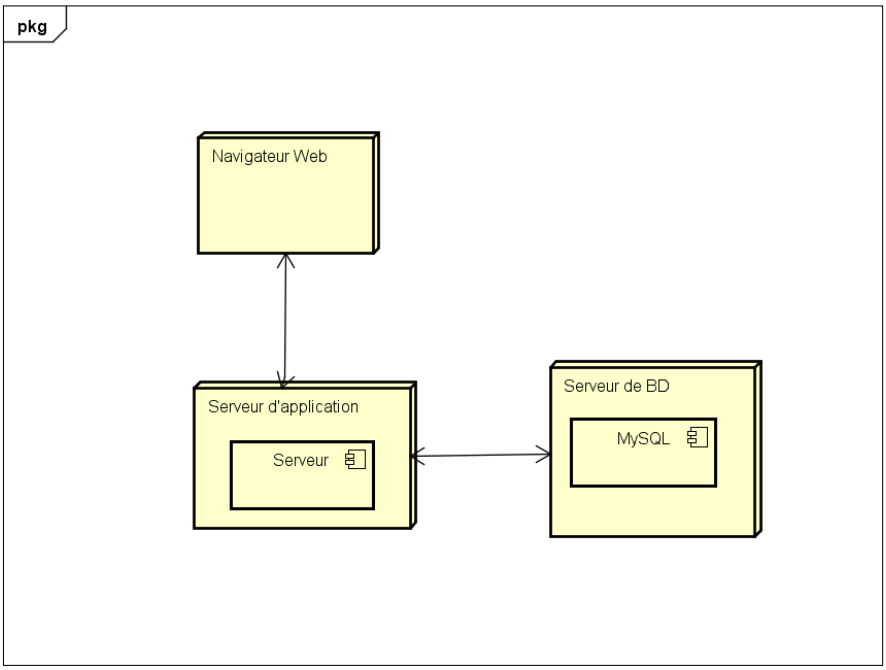
\includegraphics[scale=0.8]{images/deploiement}
	\caption{Diagramme de déploiement}
	\label{fig:deploiement}
\end{figure}

L'application si elle est mise en production sera disponible dans un premier temps sur une machine à la disposition de la personne chargée de la coordination du planning au sein du service. Les évolutions sur la plateforme pourront amener à déployer l'application sur plusieurs machines en parallèle au sein de l'hôpital. Par exemple, si l'on souhaite implémenter un système de pointage en temps réel des activités, il serait intéressant d'avoir plusieurs postes à disposition pour faciliter la tâche. Ici, nous nous focaliserons sur un déploiement sur une unique machine. 


\section{Caractéristiques des utilisateurs}
\label{sec:caracUtili}

La plateforme incorpore un système de gestion de compte afin de garantir la sécurité des données. Nous pouvons définir 2 types d'utilisateurs pour l'application.

\begin{itemize}
	\item Le personnel de soins : ils auront accès à la majorité des fonctionnalités de la plateforme (l'ajout et la recherche de patients, l'accès à leur planning personnel et au planning des patients). Ils ne pourront pas effectuer de modification sur les rendez-vous ou sur le planning en général.
	\item Administrateurs et infirmières de coordination : ils disposeront de tous les droits sur l'application. Ils pourront réaliser les mêmes opérations que le personnel de soins et auront la possibilité de gérer les ressources, gérer les activités, créer et modifier les plannings, ajouter et modifier un parcours-patient, etc.
\end{itemize}

Les utilisateurs de l'application devront s'authentifier pour pouvoir accéder aux différentes fonctionnalités et selon leur grade, ils auront accès aux éléments avec lesquels ils pourront interagir. 


\section{Contraintes de développement}

\'{E}tant donné que ce projet fait suite à plusieurs projets consécutifs et que la base de la plateforme a déjà été développée, il faudra utiliser les mêmes langages de programmes ainsi que les mêmes frameworks que lors des projets passés. Ainsi, les contraintes concernent les langages \textit{HTML}, \textit{CSS}, \textit{Javascript}, \textit{PHP}. La structure de l'application sera la même, à savoir une architecture MVC (Modèle - Vue - Contrôleur) mise en place à l'aide du framework PHP \textit{CodeIgniter}. En ce qui concerne la mise en page (\textit{CSS}), nous utiliserons \textit{Bootstrap}.

Guillaume POCHET, qui a effectué son PR\&D sur le sujet lors de l'année scolaire 2016-2017, avait réalisé un état de l'art sur les bibliothèques utilisables pour mettre en place un planning interactif \cite{pochet_outil_nodate}. À la suite de cela, il avait décidé d'utiliser la bibliothèque \textit{FullCalendar} pour constituer les plannings sur la plateforme. Nous poursuivrons avec l'utilisation de cette même bibliothèque.

De la même façon que pour les langages, il faudra reprendre la structure de la plateforme et le modèle de la base de données. Les détails concernant les structures seront dans la section suivante \autoref{sec:structure}.


\section{Description des interfaces externes du système}

\subsection{Interface matériel/logiciel}

L'application est une interface web qui fonctionne au travers d'un navigateur. Il faut donc disposer d'un ordinateur avec un navigateur web qui intègre \textit{Javascript} pour pouvoir utiliser l'application. La présence de \textit{Javascript} est nécessaire pour la visualisation du calendrier. Pour le moment, la plateforme est reliée une base de données qui doit être installée sur la machine et qui récupèrera les différentes informations nécessaires au fonctionnement de l'application. 


\subsection{Interface homme/machine}

Les utilisateurs accéderont à l'application par le biais d'un compte. L'authentification se fait à l'aide d'un nom d'utilisateur et d'un mot de passe. La création de compte est gérée par l'administrateur qui définira un type au nouveau compte créé.

On peut distinguer deux types d'utilisateurs qui ont été définis dans la \autoref{sec:caracUtili}. Par conséquent, le type d'utilisateur définira les différents onglets à afficher ou non. 

Les pages web et les onglets déjà présentes seront réutilisés lors de ce projet. Il n'y aura pas de nouvelles pages qui seront créées durant ce travail, néanmoins des modifications seront apportées aux pages actuelles, le tout en conservant l'aspect général et la charte graphique de l'application d'origine. 


\subsection{Interface logiciel/logiciel}

Comme évoqué auparavant, l'application web est liée à une base de données via \textit{MySQL}. La connexion à la base se fait au travers des classes de configurations du framework \textit{CodeIgniter}. Les contrôleurs de notre modèle MVC vont faire la liaison entre la base et l'affichage des informations. 


\section{Fonctionnalités du système}

Cette section regroupe les fonctionnalités qui vont être implémentées lors de ce projet. Les fonctionnalités déjà existantes se trouvent en \autoref{ann:foncExist}. La suite présentera les fonctionnalités qui seront ajoutées lors de ce projet. 


\subsection{Ajout de fonctions de tri lors de l'affichage des ressources}
\label{subsec:tri}

Lors de la reprise du projet, sur les premiers tests, nous avons pu observer plusieurs corrections à apporter à la plateforme. L'une d'entre elles qui m'a semblé intéressante est l'ajout de fonctions de tri lors de l'affichage des ressources. Lorsque l'on souhaite consulter le personnel, les salles ou les activités par exemple, l'affichage se fait sous forme de liste comme on peut le voir sur la \autoref{fig:affPersonnel}.

\begin{figure}
	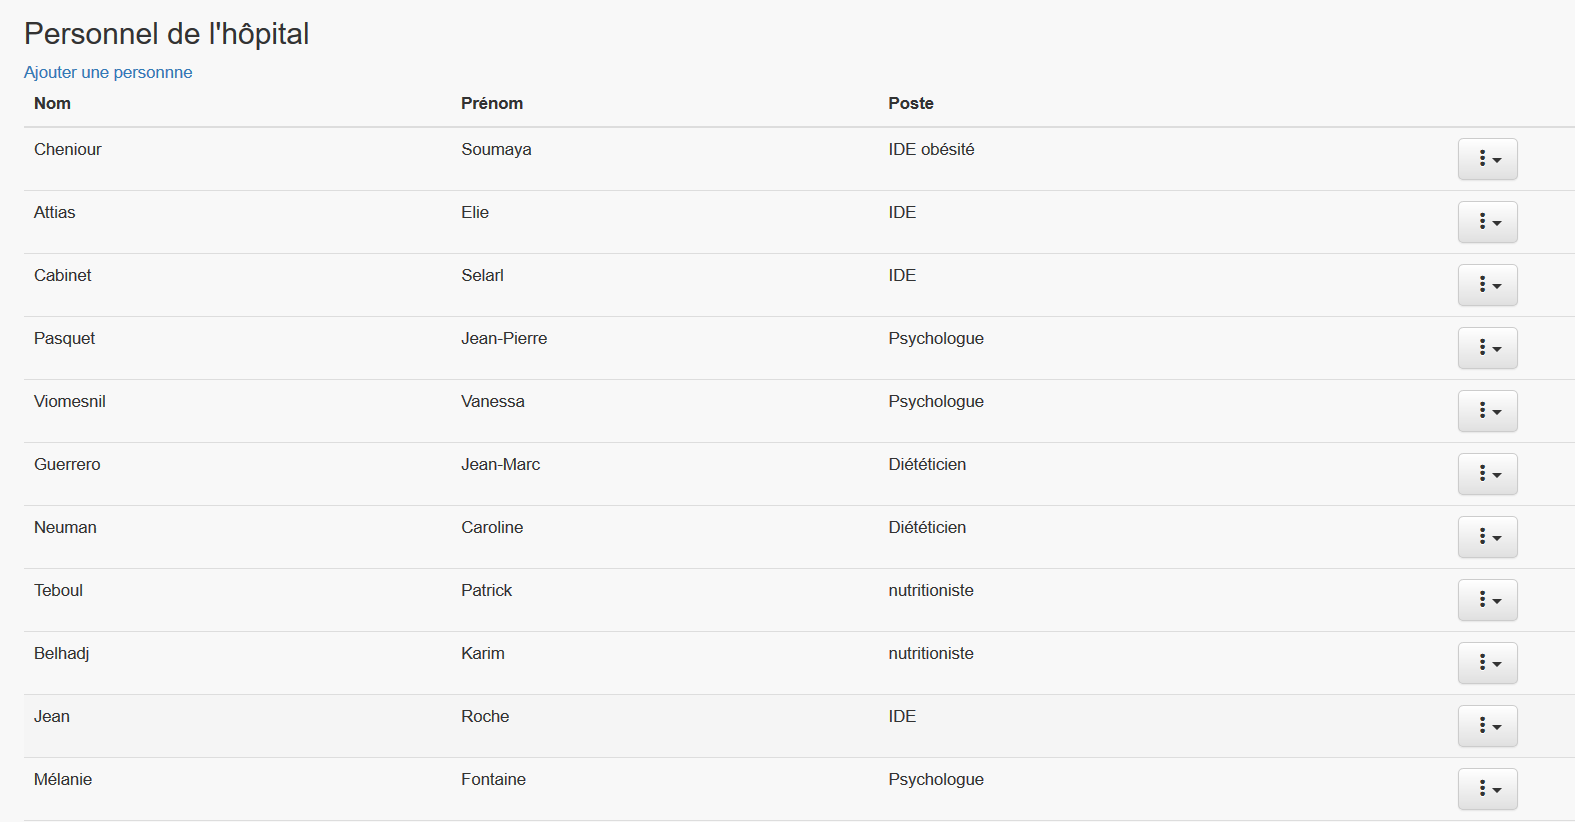
\includegraphics[scale=0.45]{images/affichage_personnel}
	\caption{Affichage du personnel sur la plateforme}
	\label{fig:affPersonnel}
\end{figure}

Cependant, dès que le nombre d'éléments dans la liste est conséquent, il devient vite difficile de trouver l'élément que l'on souhaite, d'autant plus que ces onglets n'ont pas de fonctions de recherche d'éléments.

Réaliser des fonctions de recherche peut prendre beaucoup de temps et n'est pas une priorité majeure dans notre projet. Ainsi, le compromis pour retrouver plus facilement les éléments et ne pas perdre du temps sur des fonctionnalités non prioritaires est d'ajouter des fonctions de tris sur les onglets. L'idée serait d'avoir la possibilité de trier les éléments par nom et par spécificité selon l'onglet (tri par poste pour le personnel, tri par spécialité pour les salles, etc.).


\subsection{Ajustement du planning selon les ressources sélectionnées}

Selon le même principe que l'ajout de fonctions de tri sur les onglets de gestion, un des ajustements possibles qui améliorerait l'expérience utilisateur sur la plateforme est la possibilité d'ajuster le planning selon les ressources que l'on souhaite faire apparaître.

La mise en place du planning fait partie des fonctionnalités les plus importantes mais aussi des plus complexes de la plateforme. Sur l'onglet Planification, à la reprise du projet, toutes les ressources existantes sont affichées dans le calendrier, et ainsi on peut glisser-déposer les activités non attribuées sur la ressource que l'on souhaite. Or, le nombre de ressources présentes dans l'hôpital peut vite se multiplier, et la gestion du planning devient alors très vite difficile dans ce cas.

Rendre l'affichage plus lisible et plus facile d'utilisation pour l'utilisateur n'est néanmoins pas une mince affaire car chaque information présente sur la page est importante pour faire le planning. Là où les améliorations peuvent se faire, c'est au niveau de la disposition des informations à l'écran. L'une des idées pour améliorer l'affichage est d'afficher uniquement les ressources que l'on souhaite faire apparaître à l'écran, c'est-à-dire afficher uniquement un type de personnel ou un type de salle précis. Cela permettrait de limiter les affichages à l'écran et de voir plus facilement les problèmes d'ordonnancement liés à un certain type de ressources. Par exemple, s'il y a un problème de gestion de salle (si une salle est réservée pour deux rendez-vous au même moment), en affichant uniquement les salles de l'hôpital, on peut voir directement où est le problème sans avoir à chercher parmi le flot d'informations que peut contenir la page principale. 


\subsection{Planification automatique}

Comme évoquée dans les parties précédentes de ce rapport (notamment dans la \autoref{subsec:planAuto}), l'élaboration du planning manuellement peut s'avérer très chronophage d'une part, car il faut glisser-déposer chaque activité du parcours pour chaque patient ce qui peut vite représenter plusieurs dizaines d'activités à agencer tout en prenant en compte chacune de leurs contraintes, et redondant d'autre part, car trouver un planning qui respecte les contraintes peut être long mais de plus ré-itérer cela tous les jours peut être éprouvant pour la personne en charge des plannings. La planification automatique va par conséquent être une fonctionnalité majeure de la plateforme. 

La planification automatique peut se matérialiser de plusieurs manières sur l'application. Un bouton a déjà été ajouté sur la page de planification que l'on peut voir sur la \autoref{fig:boutonPlanAuto} mais celui-ci est inactif. L'idée derrière cette implémentation réalisée lors des projets précédents est d'agencer automatiquement les activités non-attribuées sur le calendrier d'un clic sur le bouton à l'écran. 

\begin{figure}
	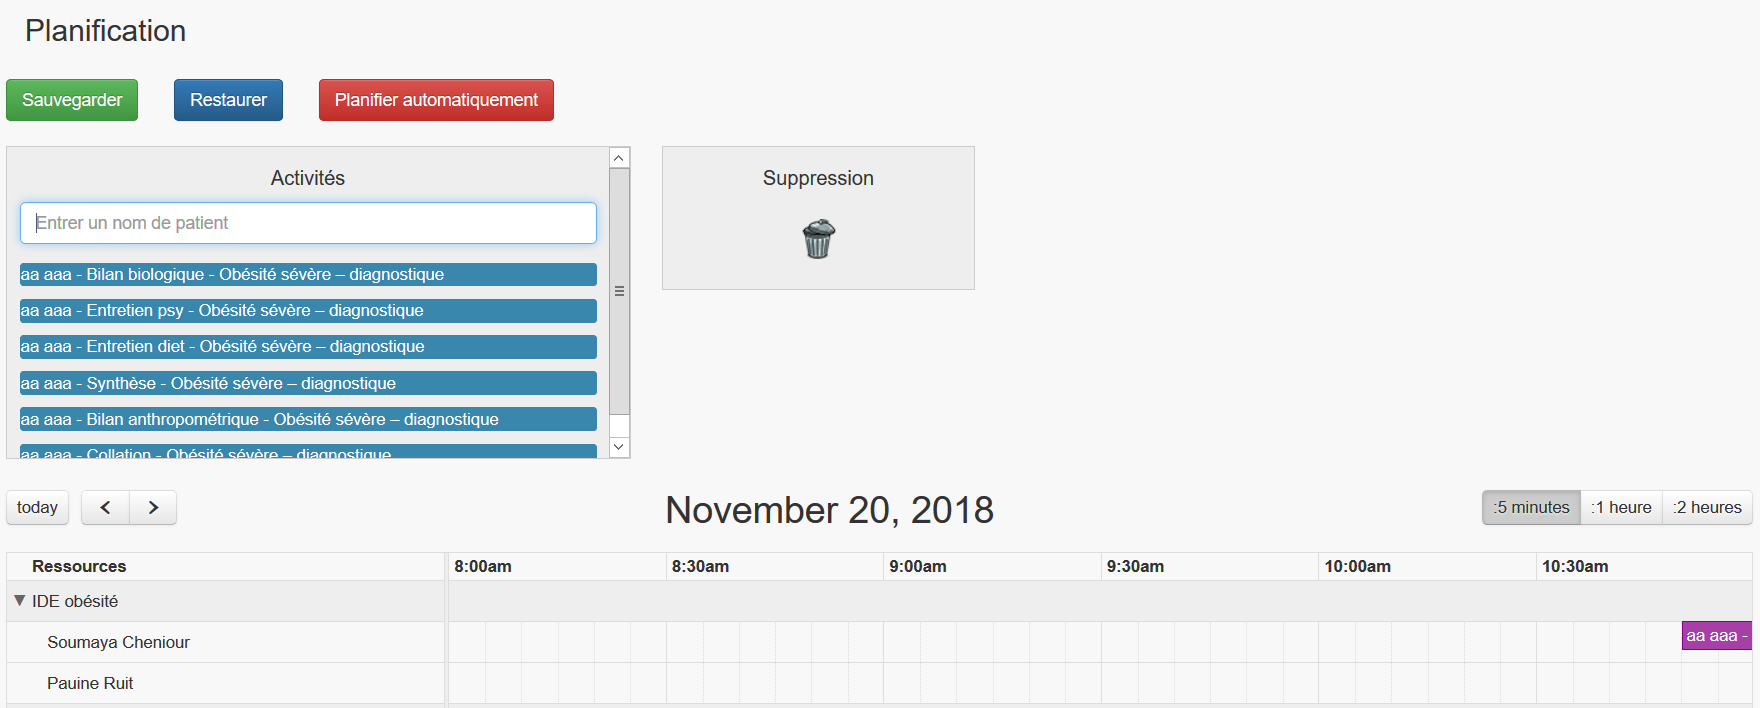
\includegraphics[scale=0.4]{images/bouton_plan_auto}
	\caption{Aperçu de la page de Planification}
	\label{fig:boutonPlanAuto}
\end{figure}

Toute la complexité de la fonctionnalité réside dans la notion que l'on souhaite donner à l'automatisme. Est-ce que l'on préfère trouver un planning qui minimise les temps d'attente des patients ? Ou alors, est-il préférable de minimiser les temps d'attente entre chaque rendez-vous pour les médecins ? Faut-il surcharger les salles quittent à \textit{over-booker} comme on peut le trouver dans les aéroports ? De nombreuses autres questions peuvent se poser à partir de ce problème.

Pour éviter les problèmes majeurs de complexité, nous allons commencer au plus simple: l'agencement patient par patient. L'idée derrière cela est d'avoir la liste des patients pris en charge le jour que l'on souhaite (comme on peut le voir pour les activités sur la \autoref{fig:boutonPlanAuto}), de sélectionner un patient et de cliquer sur un bouton qui placera chacune de ses activités du jour sur le calendrier. Le placement se fera au plus simple dans un premier temps, c'est-à-dire ajuster sur l'heure d'arrivée du patient et placer sur la première ressource disponible pour les activités. Même s'il peut y avoir des problèmes d'ordonnancement liés à cette méthode, la personne en charge pourra tout à fait ajuster l'agencement de la manière qui lui convient.

Mis en place de la sorte, même si la méthode ne donne pas un résultat parfait du premier coup, la fonctionnalité permettrait de gagner beaucoup de temps à l'utilisateur et de se débarrasser du coté redondant de l'agencement manuel. Selon l'avancement du projet, cette fonctionnalité pourra être étoffée et proposer de nouvelles options à l'utilisateur.


\section{Structure générale du système}
\label{sec:structure}

La structure générale du système est basée sur l'architecture MVC (Modèle - Vue - Contrôleur) par le biais du framework PHP \textit{CodeIgniter}. On peut voir un aperçu de l'arborescence du projet sur la \autoref{fig:arboMVC}. 

\begin{figure}
	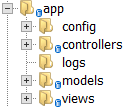
\includegraphics[scale=1]{images/arboMVC}
	\caption{Arborescence du projet}
	\label{fig:arboMVC}
\end{figure}

Sur l'arborescence, les 3 parties du MVC sont présentes ainsi qu'un dossier \textit{config} qui regroupe les classes de configuration du framework et le dossier \textit{logs} avec les classes de logger de l'application. La partie Modèle représente les données de la plateforme (patient, ressources humaines, ressources matérielles, parcours, activités, etc.). La partie Contrôleur est utilisée pour faire le lien entre les données et les différentes vues. Elle va également permettre de gérer la cohérence et l'intégrité des données. La partie Vue regroupent les pages web de l'application. 

Concernant la base de données, nous reprendrons le modèle tel qu'il a été pensé lors des projets précédents. Les explications sur l'utilité des tables et le diagramme de Gantt se trouvent en annexe (\autoref{ann:expModele} pour les explications sur les tables et \autoref{ann:modeleBDD} pour le diagramme). Des ajustements sur certains champs de la base seront apportées, notamment lors de la modification du formulaire de création de patient. 


\chapter{État de l'art}

À ce stade, le projet est avant tout un projet axé développement plutôt que recherche. La modélisation et les phases d'état de l'art sur la conception de la plateforme ont déjà été réalisées (en particulier, sur le PR\&D de Jean Coquelet \cite{coquelet_gestion_nodate}). La phase de recherche qui va nous concerner ici sera sur la question des méthodes de planification. Comme évoquée dans les sections précédentes, il s'agit d'un problème complexe où de nombreuses questions peuvent se poser. Pour éclaircir certains aspects du problème, nous allons résumer les différentes avancées de la recherche concernant les problèmes multi-ressources dans un hôpital au travers d'un article publié sur l'\textit{European Journal of Operating Research} au mois de mars 2018 \cite{marynissen_literature_2019}. Ici, nous allons voir cela au travers des démarches à effectuer pour réaliser un modèle permettant de résoudre les problèmes de planification.


\section{Présentation des problèmes multi-ressources dans un hôpital}

Dues aux constantes augmentations des frais hospitaliers et d'une demande accrue auprès des services de soins, les hôpitaux doivent trouver des moyens d'améliorer l'efficacité de leurs opérations. De nombreuses tentatives ont été réalisées ces dernières années pour développer de nouveaux plannings ou de nouvelles techniques d'admissions de patients. De ce fait, tout un panel de la recherche sur le sujet existe, que ce soit pour la planification de patient passant la nuit à l'hôpital ou non. Cependant, sur la planification, les recherches sont principalement limitées à un seul type de ressource ou un seul rendez-vous par patient. Dans la réalité, les patients doivent souvent effectuer de multiples diagnostics, consultations et/ou opérations pour être traités. De plus, traiter un seul type de ressource par patient ne correspond pas à la réalité car il est possible que le patient attende pour une autre ressource en même temps. De la même manière, un patient qui doit naviguer entre plusieurs services, implique nécessairement plus de ressources ce qui fait qu'utiliser un algorithme de planification limité à une ressource ajouterait du temps d'attente entre deux rendez-vous sur deux ressources différentes. Cela impacte le temps de traitement, et entraîne des effets négatifs sur le patient.

Ces dernières années, le nombre de travaux traitant le problème en considérant de multiples ressources est en augmentation. C'est un domaine relativement récent puisqu'aucune étude sur le sujet n'existait avant 1995. On les référence avec le terme anglais suivant : \textit{multi-appointment scheduling problems in hospitals} (MASPH). Le MASPH est défini par le problème de planification des patients qui ont besoin de rendez-vous sur certaines ressources de l'hôpital et d'optimisation des ressources de façon centralisé. Les ressources peuvent être des tests de diagnostic (scanner radio, IRM), des salles d'opérations, des médecins, etc. Chaque type de ressource peut être considéré comme un unique serveur ou comme multi-serveur. Les ressources peuvent faire partie d'un ou plusieurs services de l'hôpital. 

Le concept de MASPH est lié à plusieurs domaines de la recherche, dont notamment les suivantes : la prise de rendez-vous (\textit{appointment scheduling}), le domaine de la médecine intégrée (\textit{integrated healthcare}), les flux de patients (\textit{patient flow}), la planification de ressources (\textit{resource scheduling}) et la gestion des infirmiers (\textit{nurse rostering}). 


\section{Les niveaux de décision dans la gestion des hôpitaux}

Dans le littérature médicale, il existe 3 niveaux de décision : stratégique, tactique et opérationnel. Tout d'abord, le niveau stratégique concerne les décisions structurelles et s'adressent au long-terme en général. Dans le cas de la planification de patient, cela concerne le volume et la composition du personnel présent à l'hôpital, des ressources à acquérir et leurs localisations, et le nombre de patients à prendre en charge. Ensuite, au niveau tactique, les décisions prises sont des lignes directrices pour faciliter les décisions opérationnels. C'est à ce niveau que sont allouées les capacités pour les ressources disponibles, comme par exemple les plages horaires de disponibilité d'une machine de radiologie. Enfin, les décisions opérationnelles concernent la planification jour après jour des patients et on peut le diviser en deux parties : en différé (ou \textit{offline} c'est-à-dire les requêtes se traitent avant le jour du rendez-vous) ou en direct (\textit{online}, les évènements sont traités le jour même en direct et ne peuvent pas être prévus). 

Il est clair que tous les niveaux de décision sont importants dans le cadre des MASPH. Cependant, les principaux éléments de la recherche se font au niveau opérationnel, car bien que les niveaux stratégiques et tactiques sont nécessaires pour atteindre un résultat optimal, le niveau opérationnel constitue le cœur du problème de MASPH. 


\section{Choisir la portée du modèle}

Pour développer une méthode de planification sur de multiples rendez-vous, le premier moyen de décision est lié aux paramètres du problème, en l'occurence le service concerné, les ressources relatives aux problèmes et le type de patient concerné. 


\subsection{Le service hospitalier concerné}

Les MASPH peuvent être appliqués pour de nombreux services différents dans un hôpital et par conséquent, les problèmes de planification selon les services peuvent être très différents les uns des autres. Parmi les services où peuvent s'appliquer les MASPH, on en retrouve trois qui sont les plus étudiés dans la recherche. 

Tout d'abord, une des applications se trouve dans les services de rééducation. Ces services traitent des patients souffrant de blessures physiques ou bien d'addictions diverses. Le traitement des patients nécessitent plusieurs spécialistes et matériels venant de nombreux domaines. La visite auprès de chacune des ressources doit être planifié avec soin, ce qui est parfois une tâche difficile impliquant de nombreux acteurs. Avec une planification manuel, sans coordination, les plannings résultant sont souvent très loin de la solution optimale du point de vue du patient. Étant donnée que la rééducation est un processus long, les patients rencontrent leurs spécialistes et utilisent les ressources à de multiples reprises. Ce qui signifie que la planification dans les services de rééducation ne doit pas se focaliser uniquement sur l'agencement des tâches mais aussi sur les séries de rendez-vous successifs. Une autre difficulté dans le cadre de la rééducation est que certains spécialistes organisent des sessions groupées avec un horaire pré-défini. La rééducation peut concerner aussi bien les patients restants pour la nuit ou les patients en ambulatoire, avec dans les deux cas pour objectif, de terminer le traitement aussi tôt que possible. Pour les patients en ambulatoire, les chercheurs essaient principalement de programmer le plus de traitements possibles en un jour pour que le patient aille le moins possible à l'hôpital. En faisant de la sorte, la satisfaction des patients sera accrue et par la même occasion, le nombre de patients traités augmentera par rapport à une planification manuelle. 

La deuxième application bien référencée par la recherche concerne la planification des tests de diagnostic. Ces tests ne prennent généralement pas beaucoup de temps, il est alors possible pour un patient d'effectuer plusieurs tests en un seul jour, ce qui permettrait aux médecins de diagnostiquer plus rapidement. De ce fait, l'objectif de la planification est de minimiser le temps de réalisation de toutes les étapes de tests. Cela peut être modéliser aisément par des méthodes de recherche opérationnelle comme l'\textit{open shop}, le \textit{flow shop} ou le \textit{hybrid shop} selon les contraintes de précédence. Les tests sont suivis la plupart du temps par une consultation afin que le médecin puisse décider de la suite à donner aux traitements. Il est important de noter que tous les services de diagnostic n'utilise pas de système de rendez-vous pour planifier les patients. Certains utilisent les files d'attente pour notifier quand le patient sera admis. 

Une troisième application des MASPH se trouve dans les services d'oncologie. Bien qu'une partie de la recherche se base sur la planification des traitements de chimiothérapie et des radiothérapies, d'autres se sont focalisés sur la planification du processus de traitement entier, incluant les consultations avec les oncologues et/ou des phases de pré-traitements. Les recherches sont basées sur l'idée que les retards de traitement peuvent avoir un effet négatif sur la santé du patient. De ce fait, minimiser le temps de réalisation du traitement entier peut être très important. 

Le nombre de services où les MASPH ont été étudiés est assez limité. Cela peut s'expliquer par le fait que tous les services ne se basent pas sur une planification des patients. Par exemple, les services d'urgence utilisent davantage un modèle de file d'attente avec des priorités sur les ressources. 

\subsection{Le type de patient}

Une fois que le service a été défini, le chercheur connaît le contexte du problème et quels attributs peuvent être modifiés. Cela permet de se focaliser sur le type de patient qui seront pris en charge. Trois types de patient peuvent être identifiés: les patients en ambulatoire (\textit{outpatients}), les patients "traditionnels" c'est-à-dire qui restent la nuit à l'hôpital (\textit{inpatients}) et les patients en urgence.

Tout d'abord, les cliniques ambulatoire traitent les patients qui ne passent pas la nuit à l'hôpital. Cela signifie que le patient rentre chez lui une fois que tous les services nécessaires lui ont été administrés. Le terme "clinique ambulatoire" peut faire référence à une clinique séparée (organisée autour d'une spécialité ou sur certaines conditions médicales) ou une sous-division d'un hôpital général pour lequel les consultations sont organisées sur certains laps de temps. Les principaux challenges qui se présentent au niveau de décision opérationnel dans la procédure de planification des patients sont les incertitudes sur les temps de services et les patients ne se présentant pas aux rendez-vous (communément appelé "no-show"). L'existence des no-shows peut s'expliquer par un oubli de la part du patient ou d'un problème de transport pour aller au rendez-vous. Pour réduire l'impact de ces problèmes, il existe des heuristiques qui, en comparaison avec un planning manuel, permettent de doubler le nombre de patients programmés par jour, entraînant des revenues à la hausse pour l'hôpital.

Ensuite, pour les patients passant la nuit à l'hôpital, des ressources supplémentaires sont à prendre en compte. La ressource principale à laquelle il faut penser est le lit. Ainsi, pour planifier les patients sur les ressources, une nouvelle contrainte sur le nombre total de lits dans le système s'ajoute. De plus, le temps de séjour d'un patient est un facteur important pour la rentabilité de l'hôpital. La plupart des travaux de recherche dans ce domaine cherche ainsi à minimiser les temps de séjour. Sachant que les patients sont déjà sur place, prendre en compte les préférences du patient pour l'heure des rendez-vous n'a pas d'intérêt. Des tentatives sur des problèmes d'hospitalisation d'une semaine sur un service de rhumatologie ont été réalisées et montrent que le nombre de patients admis peut être augmenté, entraînant de meilleurs revenues pour le service.

Enfin, les patients en urgence ne font en majorité pas partie des sujets de MASPH car l'arrivée des patients n'est pas prévisible et ils doivent être traités immédiatement. Certaines exceptions existent avec des modèles qui planifient les patients dès que l'on sait quel traitement ils doivent subir. Un algorithme appliqué sur des données réelles de service d'urgence a donné des résultats améliorant les temps de réalisation des tests comparé aux temps réels.

De la cadre d'une implémentation avec tout type de patients, prendre en compte les patients en urgence est important lors de la planification des autres patients car une capacité suffisante de ressource doit rester disponible pour traiter les cas d'urgence. Si les capacités restantes ne sont pas suffisantes pour accueillir les urgences, cela entraîne un report de rendez-vous programmés qui se résulte en heures supplémentaires. Cela n'est pas désirable dans le cas des MASPH car un patient peut être attendu sur d'autres ressources par la suite, ce qui crée un cumul des retards.


\subsection{Les ressources}

Pour compléter la portée du problème, il est nécessaire de définir les ressources à prendre en compte pour modéliser au plus proche de la réalité le problème. Elles doivent être bien définies et validées car la complexité du problème en dépend fortement. Par exemple, prendre en compte les consultations avec un médecin dans le problème implique d'ajouter les disponibilités du docteur, ce qui peut faire décroître l'espace de recherche d'une solution comparé à une situation où toutes les ressources sont disponibles continuellement. Pour réduire la complexité, les chercheurs simplifient certaines suppositions, en fixant un temps de traitement pour tous les patients par exemple.


\section{Choisir ce qu'on veut optimiser}

Arrivé à ce stade, les contraintes et les paramètres du modèle sont connus du chercheur. Il est alors temps de se poser la question sur ce que l'on doit optimiser et la définition de la performance pour un hôpital. Un des points de vue est d'augmenter la satisfaction des patients. La prise en charge rapide est un élément majeur dans la satisfaction d'un patient. Bien que de nombreuses recherches partent de ce principe, un autre point de vue peut entrer en rigueur : la maximisation des profits de l'hôpital. En effet, les hôpitaux font face à de nombreuses coupes budgétaires et se doivent d'être moins dépensiers. Dans les deux cas, les MASPH ont été prouvés efficaces. Il est possible de combiner les deux en assignant des poids pour chaque fonction objectif et avec plusieurs étapes d'optimisation. De cette manière, les hôpitaux peuvent ainsi choisir ce qui leur conviennent le mieux. 


\section{Choisir comment optimiser}

À ce stade, le modèle est complet. Le but maintenant est de voir quelle méthodologie est la plus appropriée pour atteindre l'objectif. Il est important de rappeler que la communication avec l'hôpital concerné est primordial pour maximiser les chances d'implémentation du modèle dans la réalité. Ainsi, au-delà d'une technique de planification, il faut avoir aussi une stratégie de planification. Comme nous l'avons vu auparavant, on peut faire deux distinctions entre une planification \textit{online} et \textit{offline}. D'un côté, le modèle répond immédiatement avec une date et une heure pour les rendez-vous. Cela implique que la planification se fait de façon séquentielle avec les patients obtenant un rendez-vous à leur demande. De l'autre côté, les planificateurs collectent les rendez-vous et forment une liste d'attente depuis laquelle un algorithme est appliqué pour sélectionner les patients sur la liste. Choisir la stratégie de planification n'est pas une tâche aisée car les deux stratégies impliquent un mode opératoire différent pour l'hôpital. En utilisant une liste d'attente, il faut prendre en compte le fait que les patients ne doivent pas rester trop longtemps dans la liste, ce qui causerait une baisse de satisfaction du patient. De plus, dans le cas des cliniques ambulatoires, il y a une risque que les patients non traités se présentent au service d'urgence à la place car ce service traite en général tous les patients.

Pour choisir une méthodologie de planification, plusieurs options se présentent. Certaines proposent des solutions optimales, d'autres des solutions approchées. Le dilemme ici est de trouver un équilibre entre qualité de la solution et temps de calcul. Dans le cas d'une stratégie de planification \textit{online}, la méthode doit être appliquée à chaque nouvelle requête. Par conséquent, les temps de calcul doivent rester courts, limitant le modèle à l'utilisation d'heuristique, ce qui atteint rarement la meilleur solution. Pour le cas de la planification \textit{offline}, le nombre de patients à prendre en compte est plus grand, la complexité en sera ainsi accrue. Tout comme la planification \textit{online}, la recherche d'une solution optimale relève souvent d'une approche à laquelle on ne peut qu'aspirer. Les recherches traitant des méthodes optimales sont ainsi restreintes comparées aux recherches sur des solutions approchées. 


\section{Appliquer et valider le modèle}

Les dernières étapes consistent à valider le modèle pour vérifier s'il s'exécute comme prévu en utilisant des benchmarks ou des données réelles provenant d'un hôpital. Pour les résultats positifs, le modèle peut être appliqué dans la réalité. Cependant, il semble y avoir une contradiction dans les résultats de la recherche entre le nombre de modèles validés et le nombre de modèles implémentés en situation réelle. Bien qu'une partie significative de modèle dans la littérature est validée, seule une infime fraction est implémentée dans la réalité. Cela pourrait s'expliquer par une implémentation qui se fait après la date de publication par exemple. Toutefois, le fait que peu de publications ont des résultats appliqués dans la pratique a des implications sur le concept de MASPH en général. Comme peu de résultats sont disponibles, cela devient plus difficile prouver que les MASPH sont efficaces. Par conséquent, il devient plus difficile de convaincre les hôpitaux d'implémenter de nouvelles méthodes. Les études qui ont été implémentées en situation réelle ne reportent pas toujours les résultats de l'implémentation, car soit elle n'est pas complète, soit aucune donnée de performance n'est disponible avant l'implémentation. Des signes préliminaires positifs sont néanmoins apparus dans des travaux, comme dans les services d'oncologie par exemple. Peu d'études contrôlent les performances avant implémentation et rapportent les améliorations après coup. Néanmoins, afin d'appliquer une nouvelle méthodologie, il reste compliqué pour les autres chercheurs et praticiens de voir quelle méthode est meilleure qu'une autre en terme de performance. 


\part{Développement}

Cette partie est consacrée aux développements réalisés sur la plateforme. Nous allons dans un premier temps évoquer les éléments d'analyse et de conception des nouvelles fonctionnalités de l'application, puis nous détaillerons les aspects de la mise en œuvre des développements. 


\chapter{Analyse et conception}


Dans ce chapitre, nous verrons les éléments d'analyse sur les fonctionnalités de la plateforme. Ils sont séparés en plusieurs étapes correspondant au chiffrage réalisé lors des premières réunions. La gestion de projet en général ainsi que le chiffrage se trouvent en \autoref{ann:chiffrage}.

Voici les phases d'analyse que nous allons voir par la suite : 

\begin{itemize}
	\item Révision de la suppression des ressources
	\item Révision de l'onglet \textit{Plan de parcours}
	\item Révision du formulaire de création de patient
	\item Affichage du planning patient
	\item Ajout des fonctions de tri
	\item Correction des problèmes d'URL
	\item Affichage des ressources sélectionnées dans le planning
	\item Implémentation de la planification automatique
	\item Génération de jeux de données pour les tests
\end{itemize}


\section{Révision de la suppression des ressources}
\label{sec:suppr}

Les fonctionnalités de suppression des ressources ont été ajoutées lors du projet R\&D précédent sur le sujet réalisé par Yang JING. Celles-ci sont implémentées dans les onglets de gestion de la plateforme (réunis sous l'onglet "Gérer") et permettent de supprimer de la base de données les ressources qui ne sont plus nécessaires ou qui sont devenues obsolètes au fil du temps. 

L'implémentation de la suppression des ressources comporte des risques importants pour la plateforme. En effet, la suppression d'un élément peut entraîner des répercussions sur l'intégralité de l'application. Par exemple, si l'on souhaite supprimer une ressource mais que des activités sont planifiées avec cette même ressource, quelle conséquence y aura-t-il sur l'intégrité des données ? Ou encore, si on désire supprimer une activité, mais qu'un patient doit réaliser un parcours avec cette même activité, quel impact cela aura sur la planification ? Ce type de comportement sur la plateforme n'est pas souhaitable et serait même contraire au bon fonctionnement de l'application, mais une erreur de manipulation pourrait engendrer ce type d'action. 

Le problème est que, à la reprise du sujet, les boutons "Supprimer" sur la plateforme ne disposent d'aucune sécurité, ce qui peut se révéler très dangereux en cas d'erreur de manipulation. Un simple clic sur le bouton, même involontaire, entraîne la disparition immédiate de la ressource sélectionnée. Compte tenu de la dangerosité de la manœuvre sur le bon fonctionnement de la plateforme, il est nécessaire de pallier à ce problème. 

L'une des solutions à minima serait de faire apparaître un message d'avertissement lors du clic sur le bouton. Ainsi, ça permettrait déjà d'éviter les clics involontaires. Un message comme affiché sur la \autoref{fig:messSuppr} serait déjà une première étape. 

\begin{figure}
	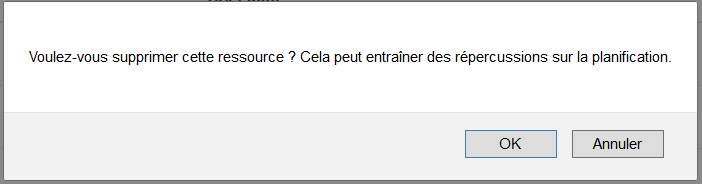
\includegraphics[scale=1]{images/messSuppr}
	\caption{Exemple de message d'avertissement en cas de suppression}
	\label{fig:messSuppr}
\end{figure}

Une autre solution plus coûteuse à mettre en place serait de cacher davantage les options de suppression. En effet, la suppression de ressource devrait une fonctionnalité plutôt rare à utiliser, une ressource devenant obsolète qu'en cas de changement de parcours. L'idée serait de placer les options de suppression sur une page séparée disponible uniquement via les paramètres du compte de la personne. Bien sûr, les suppressions peuvent être réalisées uniquement par les personnes ayant les droits adéquates sur la plateforme.


\section{Révision de l'onglet \textit{Plan de parcours}}

L'onglet "Plan de parcours" permet d'ajuster la nombre de patients qu'un parcours-patient peut accueillir par jour. La \autoref{fig:planParcours} représente l'affichage tel qu'il était à la reprise du sujet. La première remarque que l'on peut faire est que la notion de "Plan de parcours" semble floue. On ne comprend pas vraiment quel est l'utilité de l'onglet. Ajouter un texte permettant de comprendre la notion de "Plan de parcours" serait intéressant pour commencer.

\begin{figure}
	\includegraphics[scale=0.45]{images/PlanParcours}
	\caption{Aperçu de l'onglet "Plan de parcours" à la reprise du projet}
	\label{fig:planParcours}
\end{figure}

Ensuite, l'affichage des parcours se fait sous forme de liste. Pour chaque parcours, nous avons cinq lignes disposées, chacune représentant un jour de la semaine. Les parcours sont d'abord tous affichés à la suite sur l'onglet. Une liste déroulante est disponible sur le côté de la liste des parcours pour sélectionner le parcours que l'on souhaite ajuster. À première vue, l'affichage ne semble pas très intuitif pour un non-initié. Un affichage plus clair, avec des aides pour l'utilisateur, permettrait de comprendre facilement les fonctionnalités de l'onglet. 

Parmi les améliorations sur l'affichage, la mention des jours de la semaine serait intéressante. Pour le moment, comme on le voit sur la \autoref{fig:planParcours}, les jours sont symbolisés par des numéros de 1 à 5. Plutôt que d'assigner un numéro, la mention des jours en toute lettre permettrait de gagner en clarté. 

Le nombre de patients par jour et par parcours est disposé à droite de la liste. Cependant, il existe ce qui semble être une erreur sur le décompte. Il est possible d'ajuster le nombre avec des flèches disposées à droite du champ. Toutefois, il est impossible de dépasser 10 patients avec ce compteur, ce qui n'est pas normal. Une correction est donc à apporter sur ce champ. 


\section{Révision du formulaire de création de patient}

L'ajout d'un patient dans la base de données se fait à partir de l'onglet "Création" dans le menu "Patient". À partir de l'onglet, on arrive sur un formulaire à remplir pour renseigner les données du patient. L'aspect du formulaire se trouve sur la \autoref{fig:formPatient}. 

\begin{figure}
	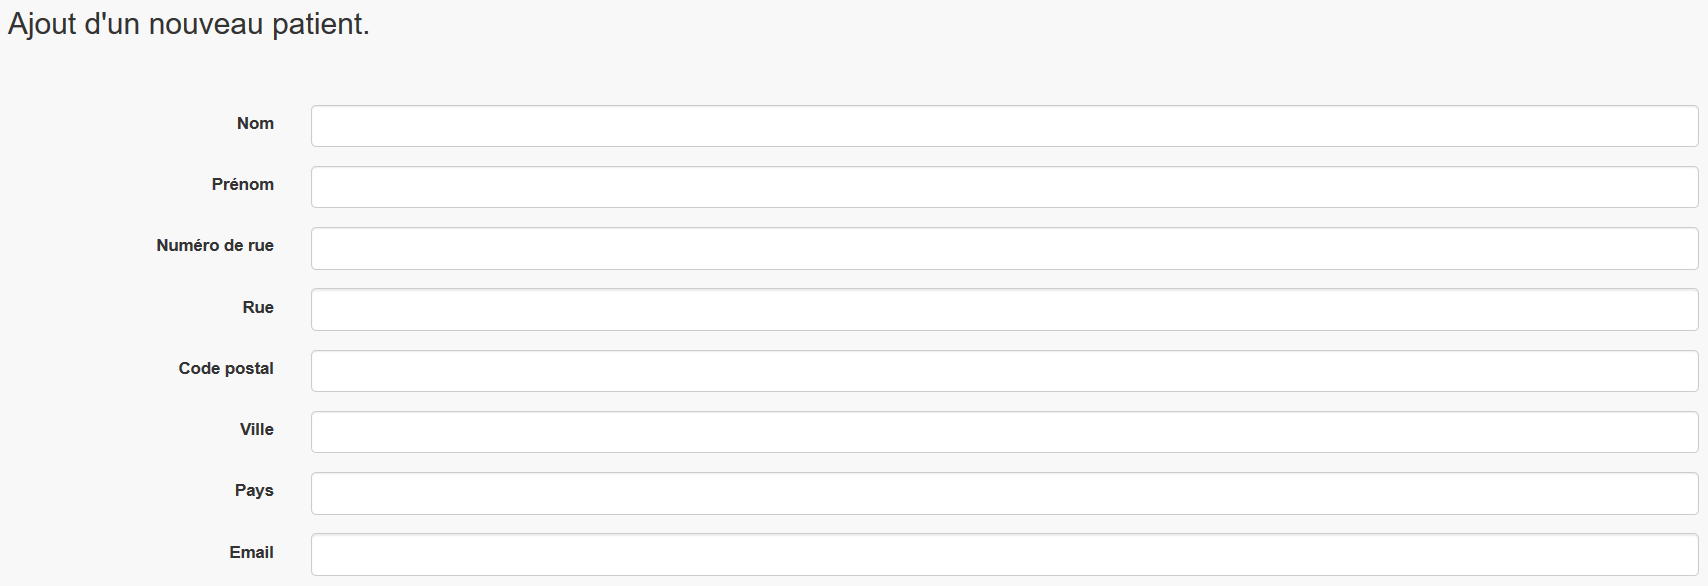
\includegraphics[scale=0.4]{images/formulairePatient}
	\caption{Formulaire de patient}
	\label{fig:formPatient}
\end{figure}

Plusieurs améliorations peuvent être effectuées sur ce formulaire, au niveau de l'affichage et des données à remplir notamment. Tout d'abord, les données à remplir vont dépendre des demandes de l'hôpital et seront quoiqu'il arrive modifiables. Néanmoins, modifier le formulaire implique de modifier la structure de la table "Patient" dans la base de données également. 

Les champs du formulaire ne disposent pas de formatage pré-disposé pour le champ en question, c'est-à-dire qu'il est possible, par exemple, de mettre des lettres sur le champ "Numéro de téléphone". L'ajout d'un formatage par défaut sur certains champs permettraient d'éviter les erreurs d'entrées dans la base de données (par exemple, une syntaxe d'adresse mail, un nombre défini de chiffres pour le numéro de téléphone et de sécurité sociale, etc.). 


\section{Affichage du planning patient}
\label{sec:planPatient}

L'affichage du planning d'un patient est une fonctionnalité qui a été présentée dans les projets précédents. Cependant, lors du test initial de la plateforme, cette fonctionnalité ne fonctionnait pas. L'affichage de planning d'un patient consiste à afficher les activités prévues pour la journée d'un patient, avec quatre informations pour chaque activité : le nom, le personnel qui s'occupera de l'activité, l'heure de début et de fin prévue. La présentation du planning est visible par la suite sur la \autoref{fig:planPatient}.

\begin{figure}
	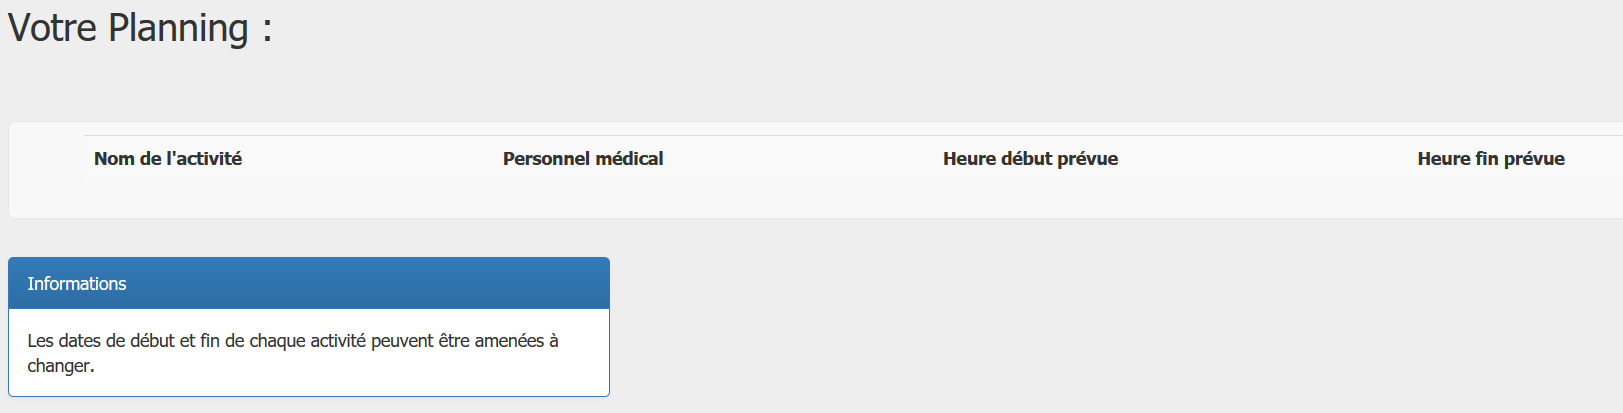
\includegraphics[scale=0.45]{images/planningPatient}
	\caption{Affichage du planning patient}
	\label{fig:planPatient}
\end{figure}

L'affichage sur le planning patient se fait à partir de la planification générale des activités. Une fois que les activités ont été positionnées sur le planning et que celui-ci a été enregistré, les activités doivent devenir visibles sur le planning du patient. 

Des éléments supplémentaires pourrait compléter cet onglet et afficher ainsi plus d'informations à l'écran. L'idée de base est d'afficher uniquement les activités prévues pour le jour même de la consultation. Ajouter un historique des consultations passées et un aperçu des activités futures seraient intéressant, tout comme proposer un visuel sur les activités prévues pour le jour-même mais qui n'ont pas été placées dans le calendrier général. 


\section{Ajout des fonctions de tri}

L'affichage des différentes ressources se fait sous forme de liste. Cependant, il peut y avoir un nombre important de ressources présentées mais il n'existe aucun tri possible pour ordonner l'affichage des entrées comme évoqué dans la \autoref{subsec:tri}. 

Par défaut, les ressources sont agencées selon leur \textit{id} dans la base de données, ce qui est une donnée invisible pour l'utilisateur. Le but serait d'ajouter une possibilité de tri pour chaque champ affiché sur la page, par exemple pour l'affichage du personnel, l'utilisateur pourra trier par \textit{Nom}, \textit{Prénom} et par \textit{Poste} en cliquant sur les titres des colonnes correspondantes comme cela se fait sur de nombreuses applications de gestion. 


\section{Correction des erreurs de redirection}

Il existe une erreur concernant la gestion des URL sur la plateforme. L'application étant une plateforme accessible via un navigateur, le parcours du site se fait au travers d'URL. Toutefois, il existe un problème au niveau de ses URL lorsque certaines actions sont effectuées. Lors de la modification d'une ressource, on la sélectionne sur l'onglet correspondant, à l'adresse \javacode{/RessourcesMat} par exemple, puis on clique sur \textit{Modifier}. On arrive sur une page de modification avec l'URL \javacode{/modif/id} avec l'\textit{id} de la ressource. Une fois que l'on confirme la modification, en cliquant sur le bouton \textit{Confirmer} de la page, on est alors redirigé vers la page des ressources en question mais avec l'adresse \javacode{/RessourcesMat/confirmModif}, comme on peut le voir sur la \autoref{fig:erreurURL}. 

\begin{figure}
	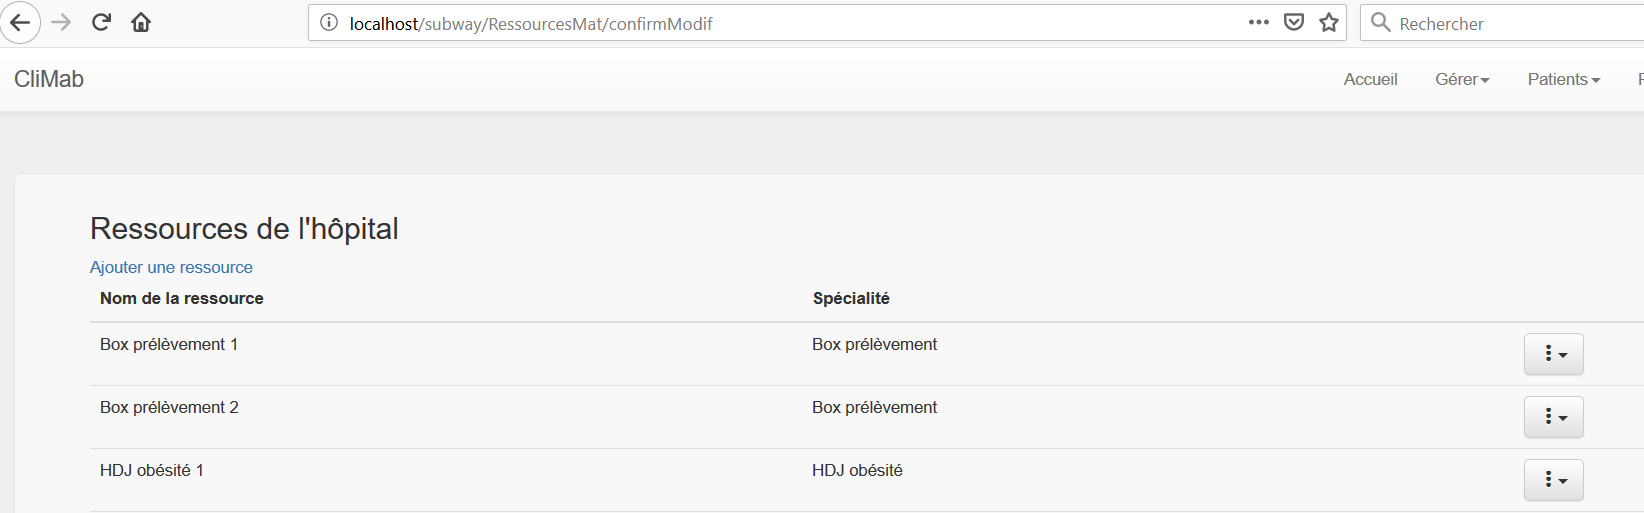
\includegraphics[scale=0.45]{images/erreurURL}
	\caption{Affichage d'une erreur de redirection}
	\label{fig:erreurURL}
\end{figure}

Ce type d'erreur peut sembler anodin, mais il peut créer des dysfonctionnements sur la plateforme, notamment en cas d'actualisation de la page ou de retour arrière. La correction de ce bug peut se faire simplement dans le code en changeant les adresses de redirection des boutons de confirmation lors de la modification d'un élément. 


\section{Implémentation de la planification automatique}

L'implémentation de la planification automatique se fera en plusieurs étapes. Tout d'abord, une refonte de certains éléments graphiques sur la page de planification sera nécessaire. La \autoref{fig:boutonPlanAuto} montre la page telle qu'elle est à l'origine du projet. La première chose que l'on remarque sur la page est la tuile centrale \textit{Suppression}. Celle-ci permet de supprimer une activité placée sur le calendrier en faisant glisser cette activité sur la zone de la tuile. Bien que l'idée de base est intéressante, l'application est moins pratique. À première vue, un utilisateur ne peut pas savoir le fonctionnement de la tuile puisque rien n'est indiqué sur la page. Ensuite, la position centrale prépondérante de la tuile n'aide pas à rendre la page ergonomique. 

Une des solutions serait de supprimer cette tuile et d'introduire un autre système de suppression. Une activité doit être placée quoiqu'il arrive, donc au lieu de faire glisser une activité que l'on souhaite enlever sur la tuile \textit{Suppression}, avoir la possibilité de la faire glisser directement sur la liste des activités qui ne sont pas placées permettrait de rendre la tuile \textit{Suppression} inutile, et ainsi elle pourrait être retirée de la page. 

Ensuite, dans le cadre de la planification automatique, nous voulons placer les activités de la façon la plus simple possible dans un premier temps, à commencer par une affectation patient par patient. Pour ce type d'affectation, il faudra ajouter une liste de patients prévu pour la journée sur la page. Celle-ci peut être placée à côté de la liste des activités, et en cliquant sur un patient, la possibilité de l'affecter automatiquement sera affichée.

Enfin, le bouton \textit{Planifier automatiquement} comme on le voit sur la \autoref{fig:boutonPlanAuto}, qui ne fonctionne pas à l'heure actuelle, resterait en place et permettrait d'affecter automatiquement tous les patients à toutes les ressources. Cette fonctionnalité sera implémentée une fois les autres éléments réalisées et sera étoffée selon le temps restant pour le projet.


\section{Génération de jeux de données pour les tests}

Sur la plateforme, on retrouve un onglet nommé \textit{Créer jeu de données}. Sur cette page, on retrouve un panneau proposant de choisir une date et un bouton avec pour intitulé \textit{Créer jeu de données} comme on le voit sur la \autoref{fig:creerJDD}. Cet onglet doit servir pour les tests de la planification. Rien n'a encore été implémenté pour le moment sur cette page.

\begin{figure}
	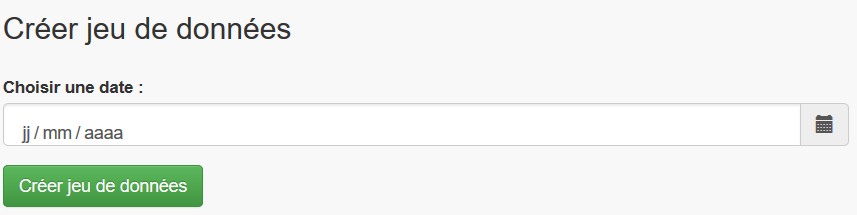
\includegraphics[scale=0.75]{images/creerJDD}
	\caption{Affichage de la page de création de jeu de données}
	\label{fig:creerJDD}
\end{figure}

La création de jeu de données va permettre de générer des patients avec des activités prévues pour la journée sélectionnée sur l'onglet. Sans ces jeux de données, le test de la planification est fastidieux puisqu'il faut créer manuellement plusieurs patients, puis leur attribuer des parcours à chacun, ce qui peut prendre plusieurs minutes. Ainsi, ce bouton ferait office de macro pour les tests. Rendre ces tâches automatiques ferait gagner ainsi beaucoup de temps lors des tests sur la plateforme. Bien sûr, cet onglet ne doit pas être accessible à tous les utilisateurs d'une part, mais aussi ne doit pas être fonctionnel en cas de mise en production. 


\chapter{Mise en œuvre}


Le chapitre suivant est consacré aux mises en place réalisées lors des phases de développement conformément aux analyses effectuées dans les parties précédentes. Seuls les éléments de mise en œuvre les plus pertinents pour le rapport seront évoqués par la suite.


\section{Ajout d'un message lors de la suppression}


% Pour la partie Suppression
%Pour afficher un message de confirmation, il suffit d'ajouter \javacode{onclick="return confirm('Etes vous sur ?');"} sur le lien de l'action ...


\section{Révision du plan de parcours}


\section{Correction sur le formulaire}


\section{Fonction de tri sur les onglets de Gestion}


\section{Planification automatique}



\chapter{Validation et Tests}


\section{Le framework Codeception}


\section{Validation }


\chapter{Qualité de code}


\section{Documentation}


\section{SonarQube}



\chapter{Avancement du projet et suite à donner}


\section{Fonctionnalités mises en place}


\section{Fonctionnalités à ajouter ou à améliorer pour la suite du projet}



\chapter*{Bilan et conclusion}

\section*{Bilan de la première partie}

À l'issue de cette première partie, nous avons pu observer les tenants et les aboutissants du projet. La plateforme comporte déjà de nombreuses fonctionnalités et l'objectif principal qui était de réaliser un outil de gestion de parcours patients a été atteint lors des précédents projets. Ici, le sujet concerne les nombreuses améliorations possibles sur la plateforme. Bien que la planification fonctionne, l'application n'est pas utilisable en production à cause d'une part, des problèmes d'ergonomie généraux, et d'autre part, de la planification qui devient vite impossible lorsque les données sont trop conséquentes.

Parmi les améliorations à effectuer, il y a dans un premier temps des améliorations générales sur la plateforme (sur l'affichage, l'ergonomie, l'expérience utilisateur en général) et dans un second temps, la planification automatique des activités. Celle-ci nécessitera la majorité du temps de développement dans la seconde partie du projet.

La suite du projet sera principalement consacrée aux développements des solutions évoquées dans les chapitres précédents. Certaines corrections ont déjà été réalisées à l'issue de cette partie, affectant l'affichage en général (corrections des fautes d'orthographe, révision de la suppression des ressources comme évoqué dans la \autoref{sec:suppr}, affichage du planning patient comme présenté dans la \autoref{sec:planPatient}). Les développements principaux, la planification automatique notamment, seront réalisées par la suite. 

\section*{Bilan de la seconde partie}


\section*{Conclusions}



\appendix

\chapter{Fonctionnalités existantes}
\label{ann:foncExist}

L'application a été réalisée par des étudiants au cours de l'année scolaire 2015-2016 puis sur les années suivantes lors d'un projet collectif et trois projets Recherche et Développement. La plateforme comporte les fonctionnalités suivantes : la gestion du personnel, des ressources matérielles, des activités, des parcours et des plans de parcours. Autre les fonctionnalités de gestion, la plateforme peut aussi créer et rechercher les patients, leur affecter des parcours et planifier les activités.


\section{Gérer les personnels}

Chaque personnel a une fonctionnalité dans l'hôpital, l'administrateur peut les modifier, supprimer et les rendre indisponible pour une période convenue.

\begin{itemize}
	\item Modifier un personnel
	\item Supprimer un personnel
	\item Mettre un personnel en indisponibilité
\end{itemize}

\section{Gérer les ressources matérielles}

Chaque ressource matérielle a un nom et une spécialité. Ces ressources correspondent aux salles de l'hôpital (les bureaux de consultation, les salles de prélèvements, etc.).

\begin{itemize}
	\item Modifier une ressource matérielle
	\item Supprimer une ressource matérielle 
\end{itemize}


\section{Gérer les activités}

Chaque activité doit avoir un nom et une durée, elle sera faite dans une certaine salle et par un ou plusieurs types de personnel.

\begin{itemize}
	\item Ajouter une nouvelle activité
	\item Modifier les activités existantes
	\item Supprimer les activités qui n'existent plus
\end{itemize}


\section{Gérer les parcours}

Un parcours se compose par plusieurs activités. Certaines activités peuvent avoir des contraintes de précedence avec d'autres. Lors de la création d'un parcours, l'agencement des activités a donc un impact important sur la planification. Pour créer un parcours, il est nécessaire de créer au préalable les activités de ce parcours si celles-ci n'ont pas encore été créées.

\begin{itemize}
	\item Ajouter un nouveau parcours
	\item Modifier un parcours
	\item Supprimer un parcours
	\item Visualiser un parcours
\end{itemize}

\section{Gérer les plans de parcours}

Dans un hôpital de jour, la capacité d'accueil les patients est limitée. Cette donnée est renseignée dans l'onglet "Plan de parcours" et peut être ajustée selon les parcours et les jours de la semaine. 


\section{Visualiser du planning}

Une fonctionnalité "Afficher planning du patient" est disponible et permet de visualiser l'heure de début et de fin de la prochaine activité du patient dans son parcours. L'affichage est restreint au jour de consultation de la plateforme (exemple: si on est le 5 du mois, on ne peut pas voir les rendez-vous planifiés pour le lendemain). Cette visualisation est accessible auprès de l'administrateur, du personnel de soins et également du patient.


\section{Affecter un patient à un parcours}

Un patient peut être affecté à un parcours en précisant les disponibilités de ce dernier. Celles-ci seront renseignées sous formes d'horaires (exemple : 8h-17h). Cette fonctionnalité est accessible à l'administrateur et aux personnels de soins. 

L'administrateur ou l'infirmière de coordination peut affecter un patient à un parcours pour une journée donnée et a la possibilité de visualiser également le nombre de patients déjà affectés sur la journée.

Lors d'un clic sur le bouton "Affecter", l'administrateur sera redirigé vers une page où il pourra choisir le patient à affecter pour la date choisie précédemment.


\section{Visualiser et modifier le planning de toutes les ressources}

L'administrateur peut visualiser et modifier en temps réel le planning de toutes les ressources et également d'une ressource en particulier. La modification peut s'effectuer de façon manuelle (en déplaçant les activités). L'administrateur doit pouvoir planifier automatiquement le planning de ses ressources pour une journée donnée. La planification automatique est l'un des sujets de ce projet et est évoquée dans les chapitres précédents. Ces fonctionnalités ne sont accessibles que pour l'administrateur. Les différentes interfaces ont été étudiées dans les projets précédents et la gestion du calendrier utilise le framework \textit{fullCalendar}.


\chapter{Modèle conceptuel de données}
\label{ann:modeleBDD}

\begin{landscape}
	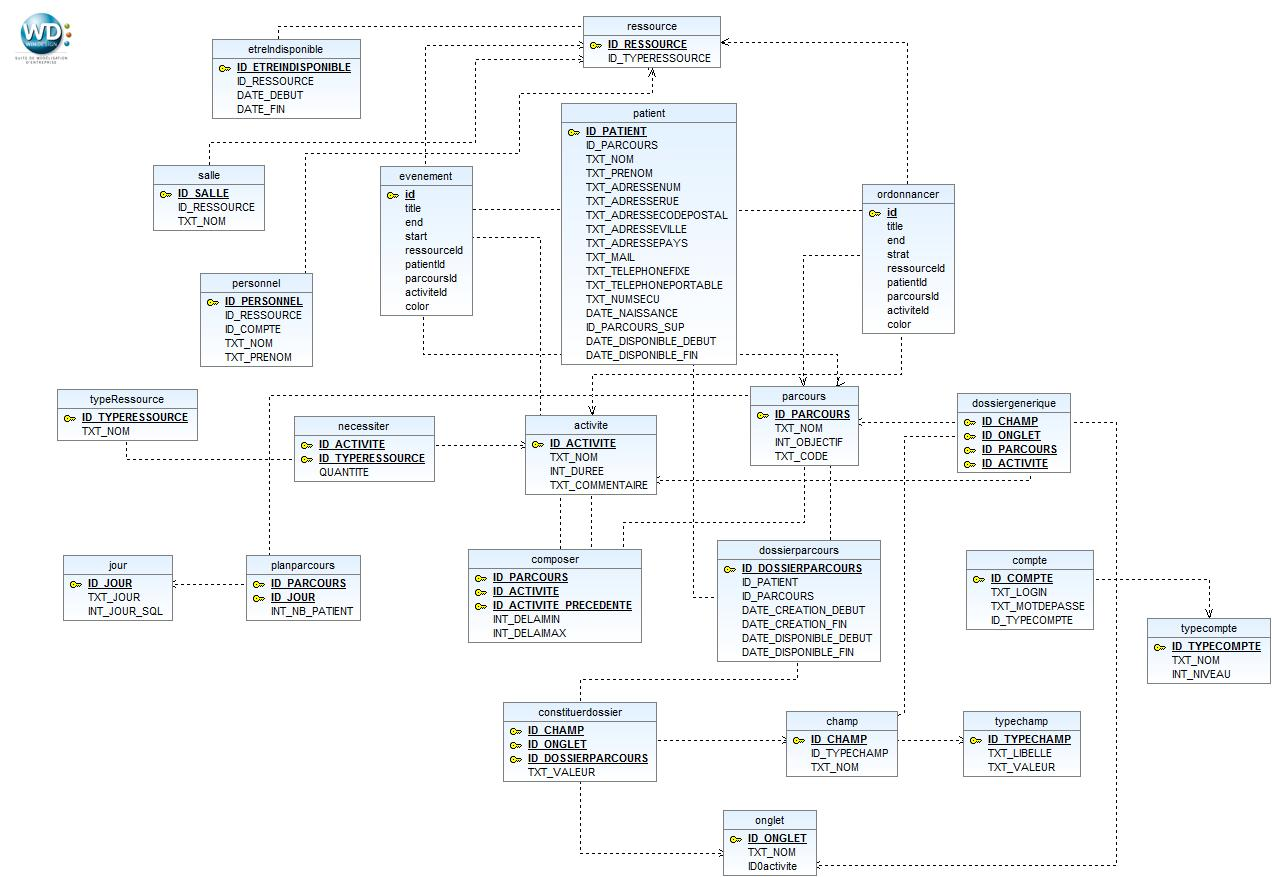
\includegraphics[scale=0.5]{images/tablesBD}
\end{landscape}

\chapter{Explications des tables du modèle}
\label{ann:expModele}


La section suivante détaille les éléments présents dans le modèle de la base de données. Les tables et la modélisation en général ont été réalisées lors des projets précédents et seront réutilisées pour le projet actuel. 

\begin{description}
	\item[Activité] : Table regroupant l'ensemble des informations concernant une activité. C'est cet élément qui constitue les parcours. Il est possible qu'une activité puisse se réaliser uniquement dans le cas où d'autres activités ont été effectuées au préalable. Cette notion de dépendance dépend du parcours en cours. Les liens entre les activités et la notion de précédence seront évoqués via la table \textbf{composer}. En plus de cela, une activité a besoin de ressources. Ce lien se fait par la table \textbf{nécessiter}.
	\item[Champ] : Table contenant l'ensemble des champs qu'il est possible d'ajouter dans un onglet d'un dossier \textit{Parcours}. À chaque champ est lié un type de champ, que nous verrons par ailleurs avec la table \textbf{typechamp}.
	\item[Composer] : Table permettant de faire le lien entre un parcours et une activité. Par l'intermédiaire de cette table, nous pouvons dire en fonction d'un parcours et d'une activité s'il y a des besoins en termes de précédence. Chaque ligne, dans cette table, a pour signification : « Pour l'activité A dans le parcours P, il faut avoir réalisé l'activité B avant, et ce dans un délai compris entre \textit{delaiMin} et \textit{delaiMax}. ». Il est important de noter qu'il est possible de mettre à « null », l'id de l'activité précédente s'il n'y a aucune contrainte.
	\item[Compte] : Table regroupant l'ensemble des comptes qu'ils soient des comptes patient ou des comptes de type ressource médicale.
	\item[Constituerdossier] : Table permettant de faire le lien entre un dossier \textit{parcours} et les informations qui le constituent. En effet, nous retrouvons pour chaque dossier \textit{parcours} et pour chaque onglet dans ce dernier, la valeur des champs le composant.
	\item[Dossiergenerique] : Table définissant, pour un parcours, les onglets et les champs que tous les dossiers parcours doivent avoir impérativement.
	\item[Dossierparcours] : Table renseignant les informations génériques d'un dossier parcours. Soit le patient associé, le parcours, dates de création et de dernière modification.
	\item[Etreindisponible] : Table regroupant l'ensemble des indisponibilités pour une ressource. Cette indisponibilité est caractérisée par une date de début et de fin, acceptant toutes les deux le renseignement de l'heure.
	\item[Jour] : Table qui contient les jours de semaine, ainsi que leurs index sous MySQL. Cette table a un enjeu au niveau des prévisions du nombre de patient par jour pour un parcours.
	\item[Necessiter] : Table permettant de renseigner les types de ressources requises pour une activité, ainsi que la quantité nécessaire.
	\item[Onglet] : Table des onglets disponibles pour constituer un dossier parcours.
	\item[Parcours]	 : Table décrivant un parcours de façon générale.
	\item[Personnel] : Table contenant l'ensemble de personnel médical de l'établissement. Chaque personne de l'hôpital a un compte, et est considéré comme une ressource.
	\item[Planparcours] : Table regroupant l'ensemble des objectifs concernant le nombre de patients pour un parcours pour un jour donné.
	\item[Ressource] : Table faisant le lien entre la table \textbf{typeressource} et \textbf{personnel} ou matériel. Ce lien	sera expliqué plus en détail avec la table \textbf{typeressource}.
	\item[Typechamp] : Table regroupant les différents type de champs qu'il est possible d'ajouter dans un dossier parcours. Elle contient également le code HTML des composants, permettant ainsi une	mise en page en accord avec les autres éléments des pages.
	\item[Typecompte] : Table utilisée pour la gestion des droits.
	\item[Typeressource] : Table contenant les types de ressource d'un point de vue activité. En effet, une activité peut avoir besoin d'un type de ressource bien caractéristique (ex : IDE obésité). C'est pourquoi nous avons un double niveau de type de ressource. Un concernant les activités (\textbf{typeressource}) et un second plus d'un point de vue logique générale (\textbf{personnel}, \textbf{matériel}).
	\item[Ordonnancer] : Table de fait de notre système. C'est la table la plus importante. Chaque ligne veut dire : « Pour le patient P qui fait le parcours Pa à la date D, il a besoin de la ressource R pour faire l'activité A de start à end. Cette table contient la planification réalisée de manière manuelle ou automatique.
	\item[Evènement] : Table identique à la table \textbf{Ordonnancer}. Elle a le même but que la table \textbf{ordonnancer} mais cette table contient la planification en cours. Cette table permet de pouvoir sauvegarder ou restaurer la planification en fonction des modifications que l'utilisateur a effectuées.
\end{description}


\chapter{Chiffrage du projet}
\label{ann:chiffrage}

\begin{longtable}{|L{12cm}|r|}
	\hline 
	\textbf{Tâches à réaliser}	& \textbf{Nombre de jours} \\ 
	\hline
	\hline 
	Révision de la suppression des ressources & 1 \\
	Révision de l'onglet "Plan de Parcours" & 1 \\ 
	Révision du formulaire de création de patient & 2 \\
	Révision de la page d'accueil & 1 \\
	Affichage du planning patient & 5 \\ 
	Ajout des tris dans les onglets d'affichage & 1 \\ 
	Correction des problèmes d'URL & 2 \\ 
	Affichage des ressources sélectionnées et test planning & 10 \\ 
	Implémentation de la planification automatique & 20 \\
	Génération des jeux de données & 3 \\ 
	Rédaction du rapport & 15 \\ 
	Préparation des soutenances & 3 \\
	\hline 
	\textbf{Total} & 64 \\
	\hline
	\caption{Chiffrage des tâches à réaliser}
\end{longtable} 


\chapter{Gestion de projet}
\label{ann:gestion}

La bonne gestion d'un projet est un élément crucial dans la réussite d'un travail, d'autant plus pour ce PR\&D car il est réalisé sur un temps plus restreint et se termine en janvier au lieu d'avril. Pour la gestion de projet, j'ai utilisé plusieurs outils divers pour gérer les tâches à réaliser au mieux. Celui qui m'a le plus servi est \textit{Trello}.

\section{Trello}

\textbf{Trello} est un outil de gestion de projet en ligne, lancé en septembre 2011, et inspiré par la méthode \textit{Kanban} de l'entreprise Toyota. Il est basé sur une organisation des projets en planches listant des cartes, chacune représentant des tâches. Les cartes sont assignables à des utilisateurs et sont mobiles d'une planche à l'autre, traduisant leur avancement. La version de base est gratuite, et c'est celle-ci que j'ai utilisé pour ordonner mon projet. J'ai principalement conservé les 3 sections disponibles par défaut : les tâches à effectuer (\textit{To do}), en cours de réalisation (\textit{Doing}) et terminées (\textit{Done}).

La \autoref{fig:trello} présente un aperçu des tâches de mon projet sur \textbf{Trello}. 

\begin{figure}
	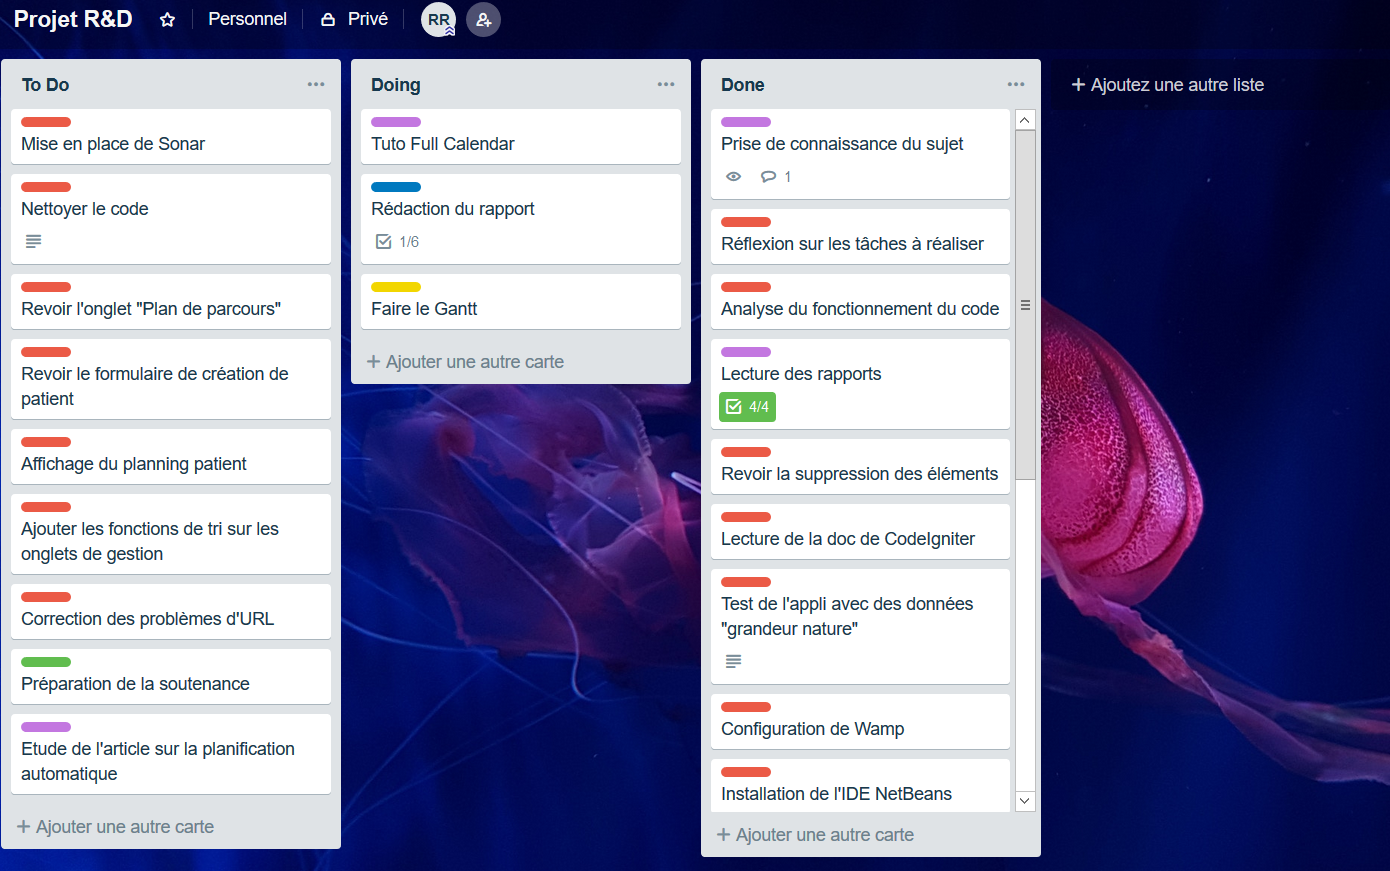
\includegraphics[scale=0.35]{images/trello}
	\caption{Aperçu de ma page \textbf{Trello}}
	\label{fig:trello}
\end{figure}

\section{Diagramme de Gantt}

Pour avoir un aperçu des tâches à réaliser dans le temps, j'ai réalisé un diagramme de Gantt avec l'utilitaire \textit{GanttProject} visible par la suite. 

\begin{figure}
	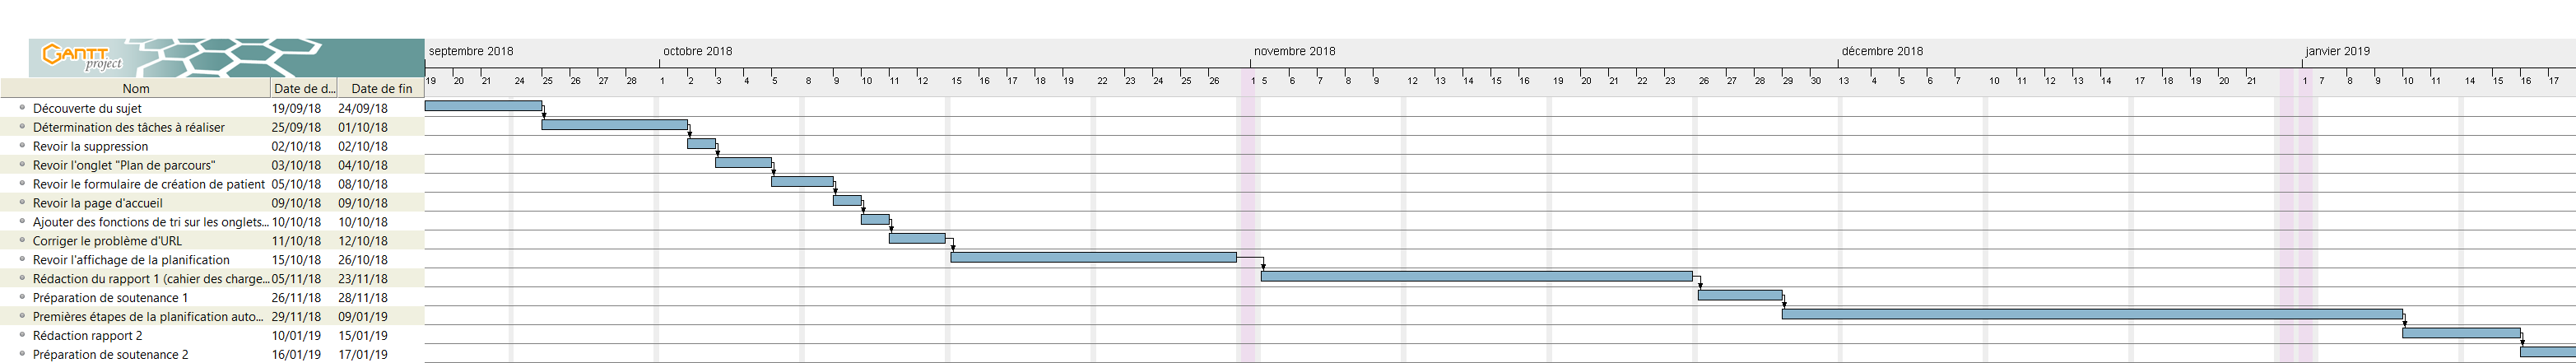
\includegraphics[scale=0.14]{images/gestion_projet}
	\caption{Diagramme de Gantt}
	\label{fig:gantt}
\end{figure}

Comme on le voit sur le diagramme, le projet va être séparé en deux parties: une consacrée aux corrections sur la plateforme et aux rédactions, tandis que la deuxième sera dédiée à la programmation de la planification automatique.

\section{Git et GitKraken}

Pour le versionning de la plateforme et du rapport, j'utilise le logiciel de gestion de versions \textbf{git}. Les sources du projet sont enregistrées sur la plateforme \textbf{GitHub}. L'application est disponible au téléchargement à l'adresse \url{https://github.com/RomainR37/ParcoursPatient}.

Pour aider au versionning, j'utilise \textbf{GitKraken} qui propose une interface graphique de l'état du projet avec Git. La \autoref{fig:gitkraken} montre un aperçu de l'interface de \textbf{GitKraken} pour mon projet.

\begin{figure}
	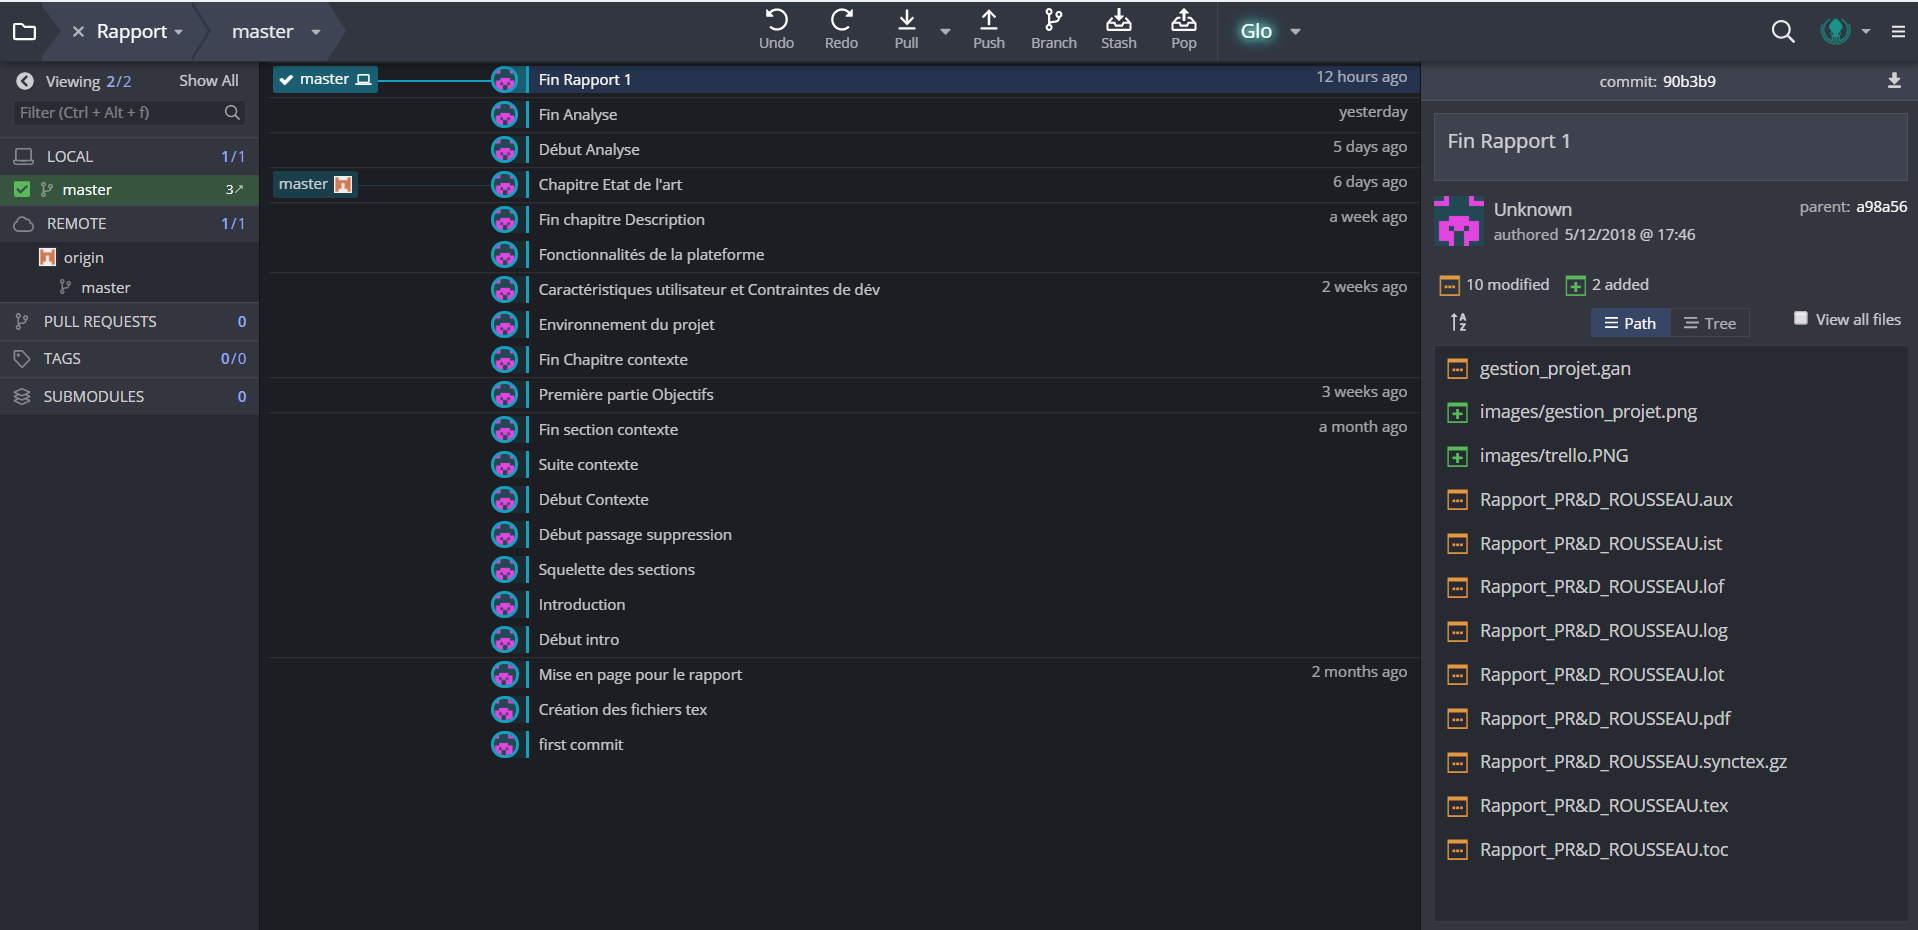
\includegraphics[scale=0.37]{images/gitkraken}
	\caption{Diagramme de Gantt}
	\label{fig:gitkraken}
\end{figure}

\chapter{Notice des livrables}

Cette partie regroupe les notices des deux livrables réalisés lors du projet: le premier le 9 janvier 2019 et le second à la fin du projet, c'est-à-dire le 25 janvier 2019.


\section{Livrable du 9/01/2019}

- Ajout d'un message d'avertissement lors de la suppression d'une ressource. Concerne les pages de l'onglet Gérer (Personnels, Ressources Matérielles, Activités, Parcours)

- Corrections sur l'onglet Plan de Parcours: affichage des jours de la semaine sous forme de texte (lundi, mardi, etc.) plutôt que par des chiffres, correction de la limite du nombre de patients affecté (limité à 10 auparavant, jusqu'à 99 maintenant)

- Ajout de règles supplémentaires sur le formulaire de création de patients: Aucune restriction sur les numéros de rue -> Numéro de rue limité à 5 chiffres, caractère numérique obligatoire, Aucune restriction sur les numéros de téléphone -> l'entrée doit contenir 10 chiffres exactement, Numéro de sécurité sociale maximum 15 chiffres -> Numéro de sécurité sociale exactement 15 chiffres.

- Fonction de tri dans les onglets Gérer: en cliquant sur les en-têtes des colonnes, la colonne correspondante est triée par ordre alphabétique. En cliquant à nouveau, la colonne est dans l'ordre alphabétique inversé. Les colonnes affectées sont 

- Correction de fautes d'orthographe diverses

\section{Livrable du 25/01/2019}


\chapter{Guide développeur}


\section{Installation du projet}


\section{Structure du projet}




\end{document}
